% !TeX encoding = UTF-8
\documentclass[a4paper, 12pt]{article}
\usepackage{geometry}
\geometry{
	a4paper,
	total={180mm,257mm},
	left=15mm,
	top=20mm,
}

%\usepackage[utf8]{inputenc}
\usepackage{graphicx}
\usepackage[dvipsnames]{xcolor}
\usepackage[style=authoryear,
hyperref,
maxbibnames=7,
backend=bibtex,
]{biblatex}
\bibliography{biblio-chapVisu}
\usepackage{hyperref}
\usepackage{xcolor}
\hypersetup{
	colorlinks,
	linkcolor={blue!50!black},
	citecolor={olive!50!black},
	urlcolor={orange!50!black}
}
\usepackage[noabbrev, french]{cleveref}
\usepackage[french]{babel}
\usepackage[babel=true]{csquotes}
\usepackage{soul} % pour \hl{}
\setlength\bibitemsep{\itemsep} % interligne entre les references
\usepackage{float} % pour localisation des tables/figures
\usepackage[belowskip=-10pt,aboveskip=8pt]{caption} % captions plus propres
\usepackage{subcaption}

% Pour tableau avec checkboxes et retour à la ligne
\usepackage{array}%
\usepackage{pifont}
\newcolumntype{P}[1]{>{\centering\arraybackslash}p{#1}}
% Pour tableau avec graphiques TikZ
\newcolumntype{M}[1]{>{\centering\arraybackslash}m{#1}}
\newcolumntype{N}{@{}m{0pt}@{}}
\usepackage{makecell}
\usepackage{tikz}
\usetikzlibrary{calc,arrows}
\newcommand{\tikzmark}[1]{%
	\tikz[overlay,remember picture] \node (#1) {};}

% Citer juste le prénom + nom d'une référence
\newrobustcmd*{\citefirstlastauthor}{\AtNextCite{\DeclareNameAlias{labelname}{first-last}}\citeauthor}


\title{Chapitre 6. Visualiser les modèles}
\author{Robin Cura\\Université Paris 1 Panthéon-Sorbonne\\UMR 8504 Géographie-cités}
\date{}
\begin{document}

\maketitle

\setcounter{tocdepth}{2}
%\tableofcontents
%\clearpage

\section*{Introduction\label{sec:intro}}

Les géographes connaissent le rôle indispensable de la cartographie pour analyser, comprendre, et décrire les espaces qu'ils étudient.
Ainsi, pour \citefirstlastauthor{pinchemel_geographie_1979} (\citeyear[\ppno~246--247]{pinchemel_geographie_1979}),
\og seule la représentation cartographique fait ressortir les organisations géographiques, les structures et les systèmes géographiques. La carte, le langage cartographique apparaissent aussi comme l'expression, comme le révélateur privilégiés de la géographie. La pensée géographique se lit dans les représentations cartographiques\fg{}.
En modélisation géographique\footnote{
Dans ce chapitre, nous référerons au terme de \og modélisation\fg{} pour désigner la modélisation informatique, formalisée sous forme algorithmique plus que mathématique, en excluant donc aussi bien la modélisation statistique, mathématique (autour de la théorie des jeux par exemple), que des types de modélisation plus habituels en géographie telles que la modélisation graphique (chorématique) ou encore la modélisation systémique qualitative (souvent formalisée sous formes de diagrammes sagittaux par exemple). Parmi les types de modélisation informatique, on notera que l'accent est ici mis sur les modèles de simulation, et qui plus est, à l'instar de la majorité du présent ouvrage, sur les modèles de simulation à base d'agents (ou simulations multi-agents, \og SMA \fg{}).
}, il n'est donc pas étonnant que la cartographie, et la visualisation de données de manière plus large, constituent des médias incontournables à l'expressivité d'un modèle.
Dans leur dernier manuel liant modélisation agents et systèmes d'information géographiques, \textcite{crooks_agent-based_2019} décrivent ainsi l'importance de la visualisation appliquée ici aux résultats de simulation :
\begin{quote}
	\og Building effective visualisations of spatial analysis and modelling outcomes, be they derived from GIS or agent-based modelling, is a vital final component of the analysis process.
	Good-quality maps and visualisations not only explain the outcomes of the analysis, but also aid interpretation by allowing observers to easily draw out insights.\fg{} \mbox{}~ \hfill \cite[117]{crooks_agent-based_2019}
\end{quote}
D'ailleurs, même quand la modélisation n'est pas géographique, on ne pourra que remarquer les parallèles sémantiques qui prédominent dans les différents outils de modélisation à base d'agents : les agents interagissent dans un \og monde virtuel\fg{}, monde qui renvoie à un espace continu, géographique, ou le plus souvent, à un espace discrétisé, composé de \og \textit{patchs} \fg{} ou de cellules, qui peuvent elles-mêmes constituer des agents (comme dans les modèles à base d'automates cellulaires par exemple). Dans le domaine des modèles à base d'agents, les agents sont généralement indissociables de l'espace support dans lequel ils évoluent, et qui peut lui-même évoluer de manière indépendante.
Les plate-formes de modélisation à base d'agents illustrent bien la forte relation entre SMA et visualisation, voire cartographie : les sites web de présentation de la majorité de ces plate-formes mettent en avant des captures d'écrans dont la plupart représentent des représentations cartographiques de modèles en cours de simulation.

Pourtant, en dépit du lien étroit entre d'une part modélisation à base d'agent et géographie, et d'autre part géographie et visualisation, la littérature scientifique liées aux SMA fait peu référence aux méthodes de représentation graphiques et en particulier cartographiques, y compris dans les articles qui s'y prêteraient le plus \autocite{lee_complexities_2015,kornhauser}.
Une analyse de littérature le montre d'ailleurs assez largement \autocite[Table 4]{angus_anarchy_2015} : dans la revue JASSS (Journal of Artificial Societies and Social Simulation), pré-dominante dans le champ de la modélisation à base d'agents en sciences sociales, les tableaux (233 identifiés), diagrammes schématiques (218) et extraits de codes (111) sont bien plus nombreux que les graphiques statistiques (43) ou les cartes (29)\footnote{Notons tout de même que les auteurs identifient 135 captures d'écrans dans ce corpus, parmi lesquelles un part non négligeable contient vraisemblablement des graphiques statistiques et des cartes.}.

Dans le monde des SMA, la visualisation de données semble donc être largement délaissée et marginale, quand bien même les chercheurs en reconnaissent l'importance \autocite{kornhauser}. De plus, dans la littérature, les visualisation sont plutôt mobilisées pour communiquer des résultats que comme outils d'analyse ou de présentation des modèles \autocite{angus_anarchy_2015}, alors que par exemple dans le domaine de l'évaluation de modèle, les chercheurs s'accordent généralement à reconnaître l'importance de la visualisation dans le processus de construction des modèles\footnote{Par exemple par l'intermédiaire des méthodes de \og \textit{face validation}\fg{}, sur lesquelles on reviendra dans la \cref{subsec:visualiser-pendant}}.

Dans ce chapitre, nous souhaitons donc présenter les avantages que peut conférer l'usage de la visualisation de données, statistiques ou cartographiques, dans la pratique de la modélisation de données géographiques.
Pour cela, il nous semble important d'établir les parallèles qui existent entre la pratique de la modélisation et celle de la visualisation.
Ces méthodes nous paraissent ainsi largement analogues, tant en termes de pratiques que de finalités.
Une fois ces parallèles établis, on pourra mettre en avant les spécificités et cas d'applications principaux de la visualisation de modèles géographiques, et ce, dans chacune des phases de conception et de vie de ces derniers.
On verra ainsi comment la visualisation peut aider à vérifier un modèle, en lui-même et vis-à-vis des hypothèses numériques sur lesquelles il est bâti, et plus généralement à procéder à son évaluation.
En extrapolant ces atouts de la visualisation d'un modèle, on pourra montrer quand et à quel point la visualisation peut se révéler utile pour comparer des modèles, pour mieux en comprendre les particularités autant que départager des modèles s'inscrivant dans une famille de modèles (voir le chapitre 4, section 4).
Après les phases de construction et d'évaluation de modèles, nous exprimerons les atouts de la visualisation dans les différentes phases de communication autour des modèles finis, c'est-à-dire en matière de présentation, valorisation et sensibilisation.
Après avoir décrit chacune des étapes de la modélisation lors desquelles le recourt à la visualisation peut s'avérer précieux, on reviendra sur les obstacles et verrous que posent les données issues de simulation au champ de la visualisation.

Ce chapitre ne constitue ni un recueil de bonnes pratiques ni un tutoriel méthodologique sur la visualisation de données. Ce champ d'étude est large, et d'autres ouvrages y sont bien plus adaptés et seront indiqués au fil de ce chapitre. Il s'adresse plutôt aux modélisateurs, débutants ou confirmés, et vise à leur donner à lire, sinon à voir, l'étendue des spectres où la visualisation de données, statistiques ou géographiques, peut procurer un intérêt majeur dans le domaine de la modélisation. En espérant que l'éventail des atouts de la visualisation permette à chacun de trouver où faire bon usage de la visualisation dans sa pratique de la modélisation.

\section{Des parallèles entre modélisation et visualisation}

Simulation et visualisation sont des domaines scientifiques majoritairement étudiés par des communautés disciplinaires très différentes et assez largement hermétiques.
Dans chacun de ces domaines, l'informatique et les chercheurs qui s'y rapportent ont un rôle prépondérant : ils conçoivent et construisent les concepts, méthodologies et outils techniques sur lesquels pourront s'appuyer les praticiens afin de modéliser les systèmes désirés ou (géo)visualiser les informations disponibles.

En se concentrant sur ces praticiens, on constate toutefois des séparations disciplinaires plus importantes.
Du côté de la modélisation, les pratiquants sont écologues, ingénieurs, archéologues, et se retrouvent assez largement sur des approches largement quantitatives de l'étude des relations entre les humains et leurs environnements (naturels ou sociaux).
Du côté des recherches en visualisation (ici au sens de visualisation de données, ou \og \textit{Information Visualisation} - \textit{InfoVis} \fg{}), la communauté est plus tournée autour d'approches créatives et artistiques, rassemblant par exemple des designers, \og data-journalistes\fg{}, ou encore les praticiens des nouvelles disciplines liées aux données, les \textit{data-scientists}.

Les géographes intéressés par la modélisation (au sens large, incluant donc les formes graphiques de modélisation) sont assez largement dispersés entre ces approches, peut-être plus pour des raisons historiques que pour des raisons d'intérêts thématiques propres
%\footnote{
%Voir par exemple la coexistence de deux Groupements De Recherche (GDR)
%, contemporains, cherchant tous deux à faire collaborer informaticiens et géographes : le GDR S4 (Simulation Spatiale pour les Sciences Sociales) autour de la simulation, et le GDR MAGIS (Méthodes et Applications pour la Géomatique et l'Information Spatiale), autour d'approches géomatiques et en partie de géovisualisation et cartographie.}
.

Pourtant, les similarités et parallèles sont nombreux entre visualisation et modélisation.
De manière générale, le lien est d'autant plus étroit qu'une visualisation est un modèle, que l'on en prenne la définition de Minsky
\footnote{
\hl{J'imagine que la modélisation aura été définie au chap 1, ou sans doute au chap 3 sinon (Lena, définition de Marvin Minksy)}
} ou une définition plus générale (\hl{renvoyer à là où la définition est donnée}).
Une visualisation est ainsi une représentation, nécessairement partielle et dédiée à une tâche, d'un ensemble de données (voir la section 2.1 du chapitre 4 par exemple).
Autant que les modèles, la visualisation implique des questions de connaissances thématiques et techniques -- et implique donc souvent l'interdisciplinarité --, mais elle est aussi concernée par des problématiques d'équifinalité (il existe potentiellement autant de manières de visualiser un jeu de données que de visualisateurs) ou d'évaluation (certaines visualisations seront ainsi plus valides que d'autres pour éclairer un aspect d'un jeu de données représentant un système).

Dans l'ensemble, on peut noter que les 9 \og principes forts\fg{} (voir \cref{tab:principes-banos}) identifiés par \citefirstlastauthor{banos_pour_2013} (\citeyear[\ppno~76--84]{banos_pour_2013}) s'appliquent au moins autant à la visualisation de données qu'à la modélisation : sans respecter leur ordonnancement ni entrer dans le détail de chacun, ces principes peuvent toutefois constituer une porte d'entrée pour dresser un portrait des similarités entre modélisation et visualisation. Qui plus est quand il s'agit de concevoir des visualisation dans le cadre d'un activité de modélisation.

\begin{table}[H]
	\centering
	\footnotesize
	{\renewcommand{\arraystretch}{1.5}%
		\begin{tabular}{|m{1.4cm}|m{7.6cm}|P{2cm}|}
			\hline
			\multicolumn{2}{|c|}{\textbf{Principe}} & \textbf{Applicable à la visualisation ?} \\ \hline
			Principe 1 & Modéliser c'est apprendre & \ding{52} \\ \hline
			Principe 2 & Le modélisateur n'est pas omni-compétent & \ding{52} \\ \hline
			Principe 3 & Les modèles de simulation doivent s'enraciner dans les données & \ding{52} \\ \hline
			Principe 4 & Le comportement de chaque modèle doit être connu de manière précise & \ding{54} \\ \hline
			Principe 5 & Le modélisateur doit cesser de proposer des solutions uniques et optimales à des problèmes complexes & \ding{52} \\ \hline
			Principe 6 & Le modélisateur n'est pas le \og gardien de la vérité prouvée\fg{}, ses modèles doivent être accessibles dans leur intégralité afin d'être reproduits & \ding{52} \\ \hline
			Principe 7 & Les modèles ne sont plus des enfants uniques & \ding{52} \\ \hline
			Principe 8 & Les modèles ont vocation à être couplés & \ding{52} \\ \hline
			Principe 9 & Les mathématiques ne sont pas le langage universel des modèles & \ding{54} \\
			\hline
\end{tabular}}
\caption{Les \og principes forts\fg de la modélisation selon \textcite{banos_pour_2013} et leur adéquation à la question de la visualisation de données.}
\label{tab:principes-banos}
\end{table}

\subsection{La visualisation comme outil d'interdisciplinarité\label{subsec:visu-interdisciplinarite}}

Les modélisateurs savent l'importance du dialogue dans la construction d'un modèle. \citefirstlastauthor{banos_pour_2013}, dans son principe 2, l'explicite ainsi : \begin{quote}
\og [Le] modélisateur doit avoir conscience du caractère fondamentalement limité de ses compétences.
Ce qui peut être perçu comme une faiblesse est pour moi une force.
Assumée, cette réalité mène naturellement à la collaboration.
De manière très générale, je dirais même que modéliser un système complexe est un acte par essence collaboratif\fg{}
\flushright\textcite[\ppno~77]{banos_pour_2013}.
\end{quote}

De la même manière, il apparaît évident que la visualisation est \og un acte par essence collaboratif\fg{}.
La visualisation n'est ainsi pas une fin en soi, mais un outil de communication au service de la transmission et de la diffusion d'un message, visuel dans ce cas.
Sans prise en compte de la manière dont une visualisation pourra être appréhendée par ses lecteurs, le risque est important de concevoir un média peu compréhensible et donc peu utile.
Les retours du public visé sont donc donc importants, d'autant plus quand la visualisation doit aider à appuyer ou à convoyer un message complexe, requérant une expertise thématique, comme c'est souvent le cas dans le cadre d'un projet de modélisation.
Dès lors, le visualisateur ne peut agir seul, de la même manière que le modélisateur ne peut se contenter de sa seule expertise.

\paragraph{Visualisation et co-construction}

La visualisation, comme la modélisation, pousse de plus non pas à une simple collaboration, mais aussi à la pratique d'une véritable co-construction tirant parti des connaissances de chacun.
Dans la conception d'un modèle de simulation, la diversité des profils des concepteurs permet d'aboutir à un modèle plus abouti, plus riche, et surtout qui vise à satisfaire les recherches thématiques et méthodologiques de ses auteurs : chacun doit y trouver son compte.
Plus les perspectives sont diversifiées, plus le modèle sera robuste dans chacun de ses aspects.

On peut illustrer ce propos à l'aide d'une expérience de co-construction interdisciplinaire -- entre géographie, géomatique, archéologie et histoire -- d'un modèle de simulation de dynamiques spatiales sur le temps long.
Ce modèle, dénommé SimFeodal (\cite{cura_transition_2017}), vise à étudier la manière dont l'espace européen a été restructuré entre le IX$^e$ et le XII$^e$ siècle, passant d'un peuplement paysan très majoritairement dispersé à une distribution spatiale concentrée en hameaux, villages et petites villes.
Chacun des membres du projet avaient en commun une volonté de tester des hypothèses d'ensembles, par exemple l'effet de polarisation des châteaux et agrégats de populations émergents, ou encore l'influence sur la fixation de la population de la mise en place du système religieux autour des paroisses.
Chacun ayant sa spécialité disciplinaire et thématique, les logiques et mécanismes du modèle ont été adoptés entre consensus et compromis, particulièrement au niveau du choix du niveau de détail de la modélisation, entre spécificité et généralité (\hl{voir chapitre 2 ?}).
Une fois le modèle construit, et afin d'en explorer le fonctionnement, la visualisation des données issues du modèle a permis de rendre compte des logiques d'ensemble, mais a aussi incité chacun des experts thématiques à vouloir observer les résultats à des niveaux différents.
Pour l'archéologue, spécialiste des paroisses dans la région étudiée, il était ainsi primordial que les résultats du modèle correspondent aux connaissances empiriques sur le nombre, la répartition spatiale et les mesures d'écartement des paroisses de l'époque.
Pour l'historien, spécialiste des communautés agraires médiévales, il était intéressant d'observer l'apparition émergente de celles-ci, et de travailler à comprendre l'avantage qu'elles conféraient à leurs membres face à la puissance du système seigneurial féodal naissant.
Pour la géographe modélisatrice, la distribution des tailles des agrégats de population constituait un enjeu important, par exemple pour déterminer si le modèle aboutissait à une hiérarchisation ou non du système de peuplement dans son ensemble.
Le visualisateur (et modélisateur), pour répondre à chacune de ces questions, a donc du concevoir une large collection de sorties graphiques illustrant aussi bien les tendances générales du modèle que les aspects thématiques spécifiques.
Pour cela, de la même manière que le modèle avait été créé dans la co-construction, les (géo)visualisations ont aussi dû être co-construites, afin de garantir aussi bien leur utilité à chaque membre que leurs adéquations aux pratiques disciplinaires de chacun en vue de les ré-utiliser par exemple dans des publications spécifiques à chaque discipline.

\paragraph{La visualisation comme outil de médiation}
De la même manière que le modèle peut constituer un outil de médiation en formalisant de manière expressive pour chacun des observations du système modélisé (en lien avec le principe 9), la visualisation remplit le même dessein.
La visualisation de données impose ainsi une transparence importante dans ce qui est représenté et dans la manière dont cela est représenté.
Là où le modèle explicite et formalise les composantes d'un système que l'on souhaite représenter, les visualisations explicitent et formalisent le modèle en lui-même.
La visualisation permet ainsi, autour d'un langage commun intuitif -- la représentation graphique --, d'expliciter les \textit{inputs}, mécanismes, comportements et \textit{outputs} d'un modèle.
Pour prendre appui sur ces derniers par exemple, il peut être utile de représenter l'évolution des attributs d'un ensemble d'agents au cours du temps.

Dans le modèle SimFeodal, par exemple, des agents \og Foyers Paysans\fg{} sont dotés d'une satisfaction, et tendent à migrer quand celle-ci est trop faible. Ce mécanisme de répulsion (\textit{push}), proche dans l'esprit de celui d'un modèle de Schelling (\cite{schelling_dynamic_1971}, ,\hl{cf. chapitre 4, voire précédents}), est completé par un mécanisme d'attraction (\textit{pull}), les agents migrants étant attirés préférentiellement par les \og pôles\fg{} (agrégats de population, églises paroissiales, châteaux\ldots) les plus attractifs.
Les détails des mécanismes régissant ces règles générales sont complexes pourraient ne relever que de particularités d'implémentation.
Pourtant, quand on cherche à étudier ce mécanisme pour étudier sous forme graphique les corrélations entre attraction d'un lieu de masse de foyers paysans attirés, de nombreuses questions émergent : la satisfaction affichée des foyers paysans est-elle calculée et enregistrée avant ou après la migration ? L'attractivité des pôles, qui dépend notamment du nombre de foyers paysans qui s'y concentrent, est-elle de la même manière représentative d'un état pré- ou post-migratoire ?
La visualisation soulève fortement ces questions car il faut trancher pour savoir ce que l'on va représenter.
De la même manière que la modélisation demande précision et explicitation de tout ce qui est modélisé, la visualisation demande précision et explicitation de la manière dont tout est modélisé (ce que \textcite{amblard_evaluation_2006} nomment \og validation interne\fg{}).

La visualisation accroît donc le rôle de médiation du modèle, en permettant une médiation sur le modèle, mais aussi une médiation plus générale pour en expliciter le fonctionnement : \citefirstlastauthor{banos_pour_2013} insiste sur le fait que le formalisme mathématique n'est pas le plus adapté à l'échange (principe 9).
Nous pourrions ici aller plus loin en ajoutant que le formalisme informatique, fait de lignes de codes ou de pseudo-code, n'est pas foncièrement plus accessible, alors que la visualisation permet de mettre sur un rapport d'égalité l'ensemble des chercheurs impliqués face à la compréhension et à la description d'un modèle.
Pour reprendre les mots de \textcite[\ppno~83]{banos_pour_2013}, quand il exprime l'intérêt du formalisme agent par rapport au formalisme mathématique : \og Je suis persuadé qu'en révélant, visuellement, le fonctionnement de méthodes même sophistiquées, et en permettant à l'utilisateur de les manipuler, d'interagir avec elles, on peut en partie faire sauter cette barrière des langages formels.
Donner une bonne intuition des méthodes est le meilleur moyen de faire en sorte qu'elles soient utilisées correctement, mais également que leurs utilisateurs se donnent à terme les moyens plus formels de les comprendre.\fg{}



\paragraph{Visualisation et interdisciplinarité}

Notons que cette égalité face à la visualisation est quelque peu trompeuse : de nombreux travaux contemporains mettent ainsi en évidence l'existence de \og\textit{visual literacy}\fg{} ou de \og\textit{data literacy}\fg{}, qui expriment les inégalités de capacité de compréhension d'informations visuelles ou d'origine numérique.
En dehors de ces inégalités qui portent souvent sur l'acculturation à la visualisation graphique, c'est-à-dire à l'habitude de lire certains types de graphiques et donc à la capacité à en comprendre rapidement le message -- les géographes doivent malgré tout \og apprendre à lire\fg{} les cartes --, on peut remarquer que les différentes cultures disciplinaires sont elles aussi porteuses d'habitudes différentes en matière de types de visualisations.

En climatologie, il est ainsi d'usage de mener une évaluation des modèles numériques de climat en en représentant les écarts aux données observées sur un graphique, nommé \og diagramme de Taylor\fg{} (d'après \cite{taylor_summarizing_2001}) qui permet de résumer trois indicateurs statistiques relatifs à cet écart en un unique graphique en deux dimensions.
Pour un géographe, ce type de représentation est pour le moins inhabituel, et demande donc une forte acculturation pour y mener intuitivement une évaluation visuelle des résultats d'un modèle.
Dans le cadre de ses recherches de thèse menée entre géographie des transports, modélisation à base d'agents et climatologie, \citefirstlastauthor{emery_ville_2016} (\citeyear{emery_ville_2016}) a mené un travail interdisciplinaire d'évaluation du modèle qu'il développait, en se basant notamment sur ce type de graphiques (\cref{fig:taylor-emery}).
Afin de rendre compréhensible ce diagramme aux membres du projet, il a donc fallu l'expliciter, c'est-à-dire détailler sa construction, la manière de le lire, et bien sûr, en donner à voir de nombreuses applications, avant que son analyse visuelle ne devienne intuitive et qu'il ne puisse ainsi constituer un outil d'évaluation adapté au modèle développé.
Cet exemple d'interdisciplinarité autour d'une représentation de modèle illustre combien la visualisation, dans le cadre d'un projet de modélisation, peut servir de catalyseur aux transferts interdisciplinaires.

\begin{figure}[H]
	\centering
	\includegraphics[width=.85\linewidth]{img/taylor_emery.pdf}
	\caption{Utilisation du diagramme de Taylor pour valider les résultats d'un modèle de simulation du traffic routier à Dijon \autocite[p. 256]{emery_ville_2016}}
	\label{fig:taylor-emery}
\end{figure}

Même quand les habitudes disciplinaires liées à la visualisation sont proches, la visualisation peut aussi permettre de nourrir un dialogue et pousser à l'explicitation.
Pour rester dans les illustrations de ces problématiques issues de la modélisation, statistique ici, on peut prendre l'exemple des courbes \og rang-taille\fg{} (voir \cref{fig:rt-gibrat}): les géographes quantitativistes, entre autres, y sont souvent confrontés et sont donc habitué à cette représentation à base d'échelles bi-logarithmiques.
Ils n'éprouveront pas de difficulté à leur lecture, et verront rapidement dans la pente de la courbe, ou de son évolution, des indices précieux sur la hiérarchie d'un système de peuplement.
Ces courbes peuvent toutefois se montrer peu parlantes pour les chercheurs issues de disciplines différentes, voir être comprises de manière inversée par certains \autocite[36]{pumain_theorie_2012}.
Ainsi, si les géographes y représentent classiquement le logarithme décimal des rangs en abscisse et celui des population en ordonnées, les économistes et physiciens inversent fréquemment ces axes. De plus, au moins pour l'exemple donné dans la \cref{fig:rt-gibrat}, on peut remarquer que les économistes emploient le logarithme népérien plutôt que le décimal, ce qui peut amener encore une fois des erreurs d'interprétation importantes.
Il convient donc d'être particulièrement prudents dans la lecture de ces courbes, et donc d'expliciter plus encore leur contenu et les résultats que l'on y lit.

\begin{figure}[H]
\includegraphics[width=.48\linewidth]{img/rt_geogan.pdf}
\includegraphics[width=.48\linewidth]{img/rt_gabaix.png}
\caption{Différentes habitudes de représentations des courbes rangs-taille.
En géographie (à gauche, \cite[fig.~2, p.~369 ]{cura_old_2017}) et en économie (à droite, d'après \cite[fig.~1, p.~740]{gabaix1999zipf}).}
\label{fig:rt-gibrat}
\end{figure}

\bigskip

Parce qu'on ne peut concevoir de visualisation de modèles sans mener une véritable collaboration, qui dans un cadre interdisciplinaire ne peut déboucher que sur des transferts thématiques et méthodologiques et des acculturations aux spécificités de chacun, la visualisation représente donc un outil d'interdisciplinarité importante.
Visualiser impose d'expliciter, aussi bien les objets représentés que les méthodes de représentations, constituant donc un formalisme commun et universel sous réserve d'une acculturation aux modes de représentation.
Et comme dans la modélisation à base d'agents, celle-ci ne requiert pas d'antécédents mathématiques importants, souvent limités en sciences humaines \autocite{banos_pour_2013}.

% Dans un modèle tel que celui de Schelling (\hl{cf. chapitre 4, voir précédents}), on observe ainsi ordinairement la satisfaction des agents afin de déterminer l'état de stabilité ou non du modèle.
% La visualisation de cette satisfaction implique, de manière pratique, de répondre à des questions précises sur la manière dont le modèle est implémenté (\og vérification interne\fg{} d'après \textcite{amblard_evaluation_2006}) : pour visualiser la satisfaction d'un agent à un pas de temps $t$ du modèle, doit-on enregistrer cette satisfaction au début du pas de temps $t$ (avant potentiel déménagement donc), ou plutôt à la fin du pas de temps ?
% Si dans le modèle de Schelling basique, où les comportements des agents sont déterministes, cela n'a sans doute pas beaucoup d'influence, ce questionnement devient prépondérant dès lors que l'on souhaite le relier à d'autres.
% Par exemple, \textcite{hatna_schelling_2012} ont proposé une extension de ce modèle, comportant de légères différences, par exemple le fait que le déplacement des agents suivent un mécanisme de type attraction (\textit{pull}) en plus du mécanisme de répulsion (\textit{push}) habituel : dans leur variante, les agents se déplacent en fonction de leur satisfaction instantannée (\textit{push}), mais aussi en fonction de l'\og utilité\fg{} des potentielles cellules d'accueil (\textit{pull}).
% Dans cette variante, les modélisateurs peuvent vouloir confirmer visuellement le bon fonctionnement de leur fonction d'utilité, et donc

\subsection{Visualisation et reproductibilité\label{subsec:reproductibilite}}

Dans son principe 6 (\cref{tab:principes-banos}), \citefirstlastauthor{banos_pour_2013} rappelle l'importance de la reproductibilité pratique et théorique des modèles.
Dans le domaine de la modélisation agent, la proposition de standard de description des modèles \og ODD\fg{} \autocite{grimm_documenting_2017} a trouvé une large adoption, même si ses auteurs insistent sur l'insuffisance de cette méthode et sur le besoin de communiquer aussi les éléments numériques d'un modèle : données en entrée, codes sources, dépendances logicielles etc.

Le monde de la visualisation n'a pas de standard aussi communément adopté, quand bien même, dans la pratique, les outils dédiés à la visualisation s'inscrivent désormais souvent dans une logique formalisée, \og grammaticale\fg{}, de conception et de spécification des visualisations : la \og grammaire graphique\fg{} (\og \textit{grammar of graphics}\fg{}, \cite{wilkinson_grammar_2006}).

\paragraph{Enracinement dans des données}

Cette manière de formaliser les modes de représentations en les \og connectant\fg{} à des données s'inscrit dans les grandes tendances actuelles de visualisation liées fortement à des données, la \og \textit{data visualization}\fg{} ou \og \textit{dataviz}\fg{}.
L'adoption de cette pratique, qui s'appuie encore largement sur des héritages des années 1960 et 1970 (John Tukey et l'analyse exploratoire de données \autocite{tukey_exploratory_1977} par exemple, ou encore autour de la sémiologie graphique de Jacques Bertin \autocite{bertin1973semiologie}, bien connue des géographes), profite considérablement de la mise à disposition d'outils informatiques libres qui s'inspirent notamment de la la grammaire graphique et permettent donc de représenter graphiquement des données de manière relativement agnostique quant aux plateformes logicielles et techniques mobilisées\footnote{
En se basant sur la grammaire graphique, on peut ainsi facilement générer ses visualisation en R, avec la bibliothèque graphique \textsf{ggplot2} \autocite{wickham_ggplot2_2016}, en Python via l'utilisation du module \textsf{Altair} \autocite{Altair2018}, ou encore générer des visualisation web (JavaScript) via \textsf{Vega} \autocite{satyanarayan_reactive_2016}.
Le code décrivant la production d'un graphique depuis chacune de ces bibliothèques est extrêmement proche, et dans tous les cas, systématiquement compréhensible par l'utilisateur de l'un ou l'autre de ces outils.
}.


Ces outils ont en commun d'être étroitement liées aux données qu'ils représentent : si les spécifications sont génériques, sans jeu de données en entrée, la représentation demeurera vide.
Cela procure l'avantage de disposer d'outils permettant de s'adapter rapidement à des mises à jour dans les données, ou encore à l'inclusion de nouveaux jeux de données -- si tant est que leur structure soit similaire --, ce qui se révèle extrêmement précieux dans un contexte de modélisation où le modélisateur exécute des centaines ou des milliers de simulation (voire des millions, cf. la partie 3.4 du chapitre 5) et peut donc ressentir le besoin d'en visualiser une large partie.
Dans une démarche de reproductibilité, cela implique aussi qu'une visualisation ne peut vivre seule, et devrait donc systématiquement être accompagnée de son code informatique, et surtout des données qu'elle donne à comprendre.

\paragraph{Reproductibilité de l'exploration visuelle}

Le chapitre 5 (section 3.4) présente des méthodes dédiées l'exploration des comportements d'un modèle de simulation, ce que \textcite{banos_pour_2013} (principe 4) jugeait comme indispensable.
Si les plate-formes mentionnées dans le chapitre précédent permettent de faire reposer ces explorations sur des pratiques documentées et reproductibles, par exemple en poussant à la communication de leur code logiciel, l'enjeu est le même pour les visualisations qui en sont issues.
Communiquer sur un modèle à l'aide de résultats graphiques non reproductibles invalide ainsi tout le processus de mise en accessibilité des modèles.

\citefirstlastauthor{reycoyrehourcq:hal-01677950} mettent ainsi en parallèle la réplicabilité d'un modèle (\cref{fig:paliers-replicabilite}, A) et celle de son exploration à proprement parler (\cref{fig:paliers-replicabilite}, B), et mènent l'expérience de reproductiblité (conceptuelle tout autant que pratique dans cette recherche) jusqu'à son terme, en proposant ainsi une mise à disposition totale de l'ensemble des éléments nécessaires à la reproductiblité d'un modèle, de son exploration, et de la visualisation des résultats issus de cette exploration \autocite[\ppno~429--433]{reycoyrehourcq:hal-01677950}.

\begin{figure}[H]
	\includegraphics[width=\linewidth]{img/reproducitiblite_exploration.pdf}
	\caption{\og Les paliers de réplicabilité d'un modèle de simulation et de son exploration\fg{}, \cite[fig.~3, p.~427]{reycoyrehourcq:hal-01677950}}
	\label{fig:paliers-replicabilite}
\end{figure}


 \subsection{Visualiser un modèle, c'est apprendre\label{visualiser-apprendre}}
 
Tout au long de son habilitation à diriger des recherches, \citefirstlastauthor{banos_pour_2013} met en avant un intérêt majeur (principe 1) à la modélisation : \og modéliser c'est apprendre\fg{}, principe qu'il reprend d'ailleurs comme titre pour la version publiée de ce travail universitaire \autocite{banos_modeliser_2016}.
Il explicite ce parti pris en inscrivant la modélisation dans une démarche itérative et abductive : \og
Modéliser est en effet un processus fondamentalement itératif qui -- et ce d'autant plus s'il est guidé par un principe d'abduction -- implique une interaction forte entre le modèle développé et la vision progressivement construite du phénomène en question
\fg{} \autocite[77]{banos_pour_2013}.
Il nous semble que le processus itératif mentionné est général à la modélisation, ne s'exprimant pas plus dans une visée abductive -- que \textcite{livet2014diversite} associent aux modèles KISS par exemple -- que dans des modèles plus empirico-inductifs (ou déductifs) tels que les modèles KIDS.
L'itération est, nous semble-t-il, au cœur de toute démarche de modélisation, que celle-ci aille des hypothèses aux concepts, des données aux hypothèses, ou encore alterne entre les trois. 

La visualisation de données de modèles s'inscrit elle aussi dans une logique très comparable, en favorisant également cette posture itérative, abductive elle-aussi \autocite[\ppno~239--240]{banos2005voie}, présente dès les fondements de l'exploration de données visuelles.

\paragraph{}
Dans le cadre d'une activité de modélisation, la visualisation permet, on l'a vu, des allers-retours thématiques et méthodologiques entre modélisateurs et thématiciens, mais doit aussi s'adapter aux différentes évolutions du modèle : les modifications des sorties, des mécanismes, de l'ordonnancement etc. ont des conséquences en matière de visualisation, puisqu'elles affectent les données sur lesquelles celles-ci se fondent.
Quand bien même les données issues du modèle ne seraient pas amenées à évoluer, on peut concevoir la réalisation d'un processus de visualisation ou d'exploration visuelle dans les mêmes termes que le processus de modélisation \autocite{andrienko2018viewing}.
La visualisation de données issues du modèle est donc en elle-même un processus itératif, et permet de plus de renforcer cette itération en permettant au modèle d'évoluer à mesure que les visualisations éclairent sa compréhension (\cref{fig:schema-va}).
La visualisation permet donc de gagner en compréhension sur le modèle, ce pour quoi elle est mobilisée à l'origine, mais aussi sur le système modélisé en lui-même : en inscrivant le processus de modélisation-visualisation dans une boucle de rétroaction qui permet de développer les connaissances sur ce qui est modélisé.

\begin{figure}[H]
	\centering
	\includegraphics[width=.8\linewidth]{img/va_models.pdf}

	\caption{Itérations et allers-retours entre modèles et visualisations pour enrichir les connaissances, traduit d'après \cite[fig.~1, p.~156]{keim_visual_2008}}
	\label{fig:schema-va}
\end{figure}

Notons aussi l'importance, en outre de la visualisation, de la manipulation, c'est-à-dire de l'interaction avec le modèle.
C'est en interagissant avec le modèle, par exemple en jouant avec les curseurs de ses paramètres, que l'on parvient à obtenir des intuitions sur les effets que ceux-ci ont sur les mécanismes du modèle.
En dehors de la géographie, c'est sur ces logiques d'interactions quasi-tangibles avec des simulations que ce sont constitués plusieurs pistes de recherche, à l'interface entre informatique, design et pédagogie, notamment autour de la communauté des \og Explorable Explanations\fg{} \autocite{case_explorable_2015}.
Pour les tenants de ces méthodes, c'est par une manipulation directe, des paramètres mais aussi des entrées et des sorties, que l'on peut comprendre comment fonctionne un système, de manière purement visuelle donc.
Comme le résume \citefirstlastauthor{victor_simulation_2009}~(\citeyear{victor_simulation_2009}), \og Model, Watch, Learn\fg{}.
Si les systèmes modélisés peuvent revêtir plusieurs formes (modèles mathématiques, physiques, ou encore statistiques), on notera une excellente expérience pédagogique autour du modèle de Schelling \autocite{schelling_dynamic_1971}, présentée sous forme d'un jeu interactif (\og Parable of the Polygons\fg{}, \textcite{hart2014parable}) et qui permet de s'emparer des leçons de ce modèle bien plus intuitivement qu'un article de recherche classique.

\bigskip 
Tout au long de cette partie, on a pu dresser les parallèles entre modélisation et visualisation en terme d'objectifs, de méthodes et de résultats obtenus.
La visualisation constituant en elle-même un modèle, ces parallèles sont prévisibles et attendus.
Appliqué à des modèles de simulation, visualiser, c'est créer \og un modèle dans le modèle\fg{} : cela permet d'enrichir une large partie des qualités intrinsèques apportées par la modélisation.
Visualiser permet ainsi d'augmenter la portée interdisciplinaire d'un modèle, d'accroître sa reproductibilité et de gagner en compréhension sur le modèle en lui-même tout autant que sur le phénomène spatial qui est modélisé.

Dans la suite du chapitre, nous montrerons maintenant quand -- dans les cycles conception d'un modèle --, et sous quelle forme, la visualisation permet en pratique de parvenir à ces aboutissements.

\section{Visualiser pour évaluer}

Dans le processus de modélisation, l'usage le plus fréquent -- ou le plus documenté -- de la visualisation s'inscrit dans les différentes phases ayant trait à l'évaluation du modèle.
Précisons d'emblée que l'on utilise ici ce terme au sens le plus large, c'est-à-dire en tant qu'ensemble des processus et techniques visant à qualifier et à quantifier la capacité d'un modèle de simulation à reproduire les éléments choisis du système modélisé.
On inscrit ainsi l'évaluation comme un terme générique correspondant aux opérations de vérification, d'accréditation \autocite{balci_verification_1997}, de validation -- interne ou externe \autocite{amblard_evaluation_2006} --, ou encore d'\og évaludation\fg{} \autocite{augusiak_merging_2014}.

Il est d'usage de subdiviser la pratique de l'évaluation en deux grandes catégories liées à l'objet qui doit être évalué : soit la correspondance d'un modèle implémenté au modèle empirique, théorique ou conceptuel sur lequel il repose (validation interne\footnote{
Selon l'expression consacrée : \og Model verification deals with building the model~\textit{right}.\fg{} \autocite[\ppno~165]{balci_validation_1994}
}), soit la correspondance entre le modèle implémenté et les faits stylisés du système qu'il cherche à reproduire (validation externe\footnote{
\og Model validation deals with building the \textit{right}~model.\fg{} (\textit{ibid.})
}).
Ce chapitre ne porte toutefois pas sur l'évaluation de modèles, et comme la visualisation constitue l'une des méthodes\footnote{
Notons que dans la typologie des méthodes d'évaluation de \textcite{balci_verification_1997}, plusieurs méthodes font appel à la visualisation de données. On ne reprendra pas ici la distinction que fait l'auteur.
} d'évaluation, on ne suivra pas cette distinction.
On y préfèrera un découpage chronologique -- au moins en termes d'avancée du modèle, la chronologie pure étant mise à mal par le caractère itératif de la modélisation --, en relevant les phases de la modélisation où la visualisation peut constituer un atout important.
Il s'agira donc de décrire les potentialités de la visualisation appliqué avant, pendant, et après la simulation.

\subsection{Visualiser avant de modéliser}

Certains modèles font reposer leurs hypothèses sur des études empiriques centrées sur des données statistiques (principe 3 du \cref{tab:principes-banos} par exemple).
Dans ces cas là, la visualisation permet de vérifier les résultats de traitements numériques qui pourraient être inexacts, voir invalides, faute d'un observation visuelle assez fine des données.
De nombreux analystes ont ainsi tendance, par soucis de rapidité, à se contenter d'examiner les résultats numériques résultant d'agrégations ou de modélisations de données, et de repartir de ces résultats pour formuler leurs hypothèses.
C'est toutefois oublier que ces modélisations numériques, de par la réduction de dimensionalité qui en constitue le cœur, ont nécessairement pour effet d'appauvrir les données sous-jacentes, de les résumer en un faible nombre d'indicateurs, ce qui ouvre dès lors la place à des interprétations abusives.
Notons que le problème n'est pas exactement nouveau : c'est face au même constat qu'est apparu un champ majeur des statistiques : l'analyse exploratoire de données :
\begin{quote}
	\og
	Once upon a time, statisticians only explored.
	Then they learned to confirm exactly--to confirm a few things exactly, each under very specific circumstances.
	As they emphasized exact confirmation, their techniques inevitably became less flexible.
	The connection of the most used techniques with past insights was weakened.
	Anything to which a confirmatory procedure was not explicitly attached was decried as "mere descriptive statistics", no matter how much we had learned from it.\textelp{}\\
	\textbf{Today, exploratory and confirmatory can --and should-- proceed side by side.}
	\fg{} \mbox{}~ \hspace{2.5cm} \cite[Préface, \ppno~vii]{tukey_exploratory_1977}
\end{quote}
\medskip
Dans cet ouvrage, \citefirstlastauthor{tukey_exploratory_1977} introduit notamment la représentation de formes de distributions à l'aide de \og \textit{box plots}\fg{} (\og boîtes à moustaches\fg{} selon l'usage francophone) qui permettent en particulier de repérer les \textit{outliers} (valeurs aberrantes) et de les isoler des formes plus générales d'une distributions (quartiles et déciles).
C'est d'ailleurs tout l'enjeu de la visualisation que de pouvoir communiquer rapidement un message plus complet qu'un tableau ou des mots ne sauraient exprimer aussi brièvement.
Dans la même lignée, on peut citer les travaux de \textcite{anscombe_graphs_1973}, qui montre que les indicateurs relatifs aux valeurs centrales et de dispersions de même que les indices de corrélation peuvent inciter en erreur en faisant passer pour similaires des nuages de points très différents (voir \cref{fig:anscombosaurus}).

\begin{figure}[H]
	\centering
	\includegraphics[width=\linewidth]{img/anscombosaurus.pdf}
	\caption{Différents jeux de données ayant des moyennes, médianes, variances et coefficients de corrélations identiques. D'après \textcite{matejka_same_2017} et \textcite{cairo_download_2016} (pour la figure du dinosaure \og \textit{Anscombosaurus}\fg{}).\\
	NB : Le segment bleu correspond à la droite de régression de la corrélation : elle est quasi-identique (et faible) dans tous ces jeux de données.}
	\label{fig:anscombosaurus}
\end{figure}

Notons que cette figure illustre un autre biais statistique connu que la visualisation peut aider à débusquer : le jeu de données \og \textsf{slant\_up}\fg{} montre ainsi une corrélation globalement négative (la droite de régression a une pente négative), alors que le jeu de données semble, visuellement, composé de cinq sous-ensembles qui auraient chacun, indépendamment, une pente positive.
C'est le paradoxe de \textcite{simpson_interpretation_1951}, qui peut avoir des effets extrêmement pervers en modélisation agent : si la tendance agrégée est inverse aux tendances individuelles, et sans vérification de ces biais statistiques, le modélisateur peut concevoir un mécanisme qui serait inverse aux connaissances et observations empiriques.

\bigskip
Ces quelques exemples illustrent l'importance de la visualisation quand on est amené à traiter avec des données statistiques, mais aussi dans le cas spécifique de la modélisation, où différents biais et effets statistiques (on pourrait en outre citer le \textit{MAUP} de \textcite{openshaw1984modifiable} en potentiel paradoxe spatial) peuvent amener les modélisateurs à concevoir leur modèle de manière erronée quand aux comportements individuels ou agrégés des agents.
La visualisation de l'ensemble des données permet d'améliorer la vérification des phénomènes modélisés, et enrichit donc les étapes préalables à la modélisation.


\subsection{Visualiser pendant la simulation\label{subsec:visualiser-pendant}}

Dans le processus d'évaluation de modèle, parmi les phases faisant appel à la visualisation, la plus connue est sans doute l'étape de \og \textit{face validation}.
Cette étape est ainsi l'une des premières pratiques recommandées pour garantir une certaine plausibilité, d'apparence tout au moins, au modèle implémenté (voir \cref{fig:schema-kluegl}).
La \textit{face validation} consiste en effet à vérifier visuellement, en prenant appui sur des intuitions sur le comportement attendu, la plausibilité du modèle, c'est-à-dire l'adéquation potentielle entre d'une part le déroulement et l'issu d'une simulation, et d'autre part les connaissances expertes que l'on possède sur le système modélisé.

\begin{figure}[H]
	\centering
	\includegraphics[width=\linewidth]{img/Schema_Kluegl_traduit.pdf}
	\caption{Les phases classiques de l'évaluation d'un modèle de simulation.
		Traduction d'après \textcite[fig.~1, \ppno~42]{klugl_validation_2008}}
	\label{fig:schema-kluegl}
\end{figure}

\medskip
\citefirstlastauthor{klugl_validation_2008} (\citeyear[\ppno~41--42]{klugl_validation_2008}) détaille ce processus en y inscrivant trois composantes, toutes basées sur la création de visualisations du modèle :\\
\begin{itemize}
	\item \textbf{Évaluation du déroulement (\textit{Animation Assessment})} Évaluation du déroulement d'une simulation dans son ensemble.
	Il s'agit ici de juger de la plausibilité des dynamiques (à l'échelle du système dans son ensemble, ou de composantes de celui-ci) reproduites dans la simulation, via une observation en direct de la simulation.
	
	\item \textbf{Évaluation des sorties (\textit{Output Assessment})} Cette approche consiste plutôt à une évaluation qualitative des sorties produites par la simulation.
	Cela peut prendre la forme de vérification des valeurs (approche que l'on retrouve dans les méthodes d'évaluation plus formelles, via une automatisation de ces types d'évaluation) par un expert, mais aussi d'analyse des co-variations et évolutions temporelles de différents indicateurs de sortie.
	L'évaluation des sorties peut être appliquée sur le système modélisé dans son ensemble, mais aussi au niveau des types d'agents mobilisés.
	
	\item \textbf{Évaluation \og immersive\fg{} (\textit{Immersive Assessment})} Il s'agit ici d'évaluer le modèle au travers de la vraisemblance des actions et réactions individuelles des agents qui y interagissent. L'accent est donc mis sur la plausibilité du comportement des agents (niveau micro), plus que sur celle des dynamiques macroscopiques résultantes.
\end{itemize}
\medskip
Les différentes plate-formes de modélisation à base d'agents mettent en avant les deux méthodes qui s'effectuent \og en direct\fg{} de la simulation, c'est-à-dire l'évaluation du déroulement et l'évaluation immersive (voir \nameref{sec:intro}).
Les outils de visualisation proposés par ces outils sont ainsi pensés pour être aussi intuitifs que possibles et donner lieu à des visualisations du modèle dès le début de son implémentation, par exemple dans les phases de prototypage.
Ces visualisations comportent presque systématiquement une -- ou plusieurs (\cref{fig:gui-gama}) -- carte du \og monde\fg{} modélisé où l'on représente les agents et où l'on peut donc visualiser leurs déplacements et l'évolution de leurs attributs, par exemple en les représentant sous la forme de symboles proportionnels (attributs quantitatifs) ou en affectant des symboles différents aux agents (attributs qualitatifs) (\cref{fig:gui-netlogo}).
Ces cartes sont souvent complétées par des graphiques statistiques, figurant par exemple l'évolution d'un indicateur au cours du déroulement d'une simulation (les différents graphiques occupant les parties de gauche dans les \cref{fig:gui}).

\begin{figure}[H]
\centering
\begin{subfigure}{.5\linewidth}
	\centering
	\includegraphics[width=\linewidth]{img/Accessim_GUI.png}
	\captionsetup{width = .9\linewidth}
	\caption{Modèle AccesSim \autocite{delage:halshs-00607754}, développé avec la plateforme NetLogo \autocite{tisue_netlogo_2004}.}
	\label{fig:gui-netlogo}
\end{subfigure}%
\begin{subfigure}{.5\linewidth}
	\includegraphics[width=\linewidth]{img/gama-3D.png}
	\captionsetup{width = 1\linewidth}
	\caption{Modèle BSNM (Brown plant hopper Surveillance Network Model, \textcite{truong_modeling_2012}), développé avec la plateforme Gama \autocite{taillandier_building_2018}.}
	\label{fig:gui-gama}
\end{subfigure}
\caption{Interfaces graphiques de deux modèles de simulation géographiques illustrant différentes visualisations (carto)graphique dédiées à l'observation du déroulement de modèles de simulations.}
\label{fig:gui}
\end{figure}

La visualisation \og en direct\fg{} (\textit{online} chez \textcite{grignard_agent-based_2017}) est nécessairement contrainte par l'espace visuel présenté au modélisateur.
A mesure que l'on souhaite raffiner l'observation des comportements du modèle, on tend ainsi à ajouter de nouvelles visualisations, démultipliant le nombre d'indicateurs à surveiller au cours d'une simulation.
Il peut donc être utile de mener des observations \textit{a posteriori}, c'est-à-dire en visualisant différents indicateurs -- et leur évolution -- une fois la simulation achevée.
Les plateformes de simulation adoptent face à ce besoin récurrent des stratégies différentes.
Certaines (Gama par exemple) proposent de multiplier les onglets dédiés à la visualisation, parmi lesquels on pourra alors alterner afin de mener une \textit{face validation} plus poussée (\cref{fig:gui-gama}).
Cela permet de ne pas surcharger l'affichage d'ensemble du modèle et de lui conserver un rôle de synthèse.
D'autres plateformes (NetLogo\ldots) proposent un mécanisme extrêmement pratique qui consiste à pouvoir \og rejouer\fg{} une simulation, c'est-à-dire à permettre au modélisateur de se déplacer dans les pas de temps une fois l'exécution du modèle achevée.
Ainsi, on pourra se concentrer sur quelques indicateurs, voir en ajouter de nouveaux de manière interactive quand la plateforme le permet.


\bigskip

Dans tous les cas, et parce que la modélisation est une tâche fortement itérative, il est fortement recommandé de sauvegarder, dans les sorties d'un modèle, les états des différents agents à chaque pas de temps de simulation.
Cela permet d'une part de mener des analyses postérieures plus approfondies (mobilisant par exemple des méthodes d'analyse spatiale non implémentées dans les plateformes génériques de modélisation agent), mais aussi d'autoriser un retour ultérieur sur des simulations passées, quand bien même de nouvelles versions du modèle auraient été implémentées entre temps.

\subsection{Visualiser après la simulation \label{subsec:visualiser-apres}}

La visualisation \textit{a posteriori} est importante dans l'évaluation d'un modèle : 
si tant est que l'ensemble des éléments (agents et attributs par exemple) aient été sauvegardés pendant l'exécution d'une simulation, elle permet ainsi de revenir à tout moment sur les résultats d'une simulation, que ce soit pour en préciser l'analyse ou encore pour en comparer les résultats avec ceux d'autres simulations.

\paragraph{Analyse des résultats d'une simulation}

Au niveau de la précision de l'analyse, on peut mentionner différents usages en modélisation géographique.
Les plateformes de modélisation à base d'agents mettent à disposition de plus en plus de méthodes d'analyse statistiques et géostatistiques, de possibilités de (géo)visualisation et d'outils intégrés d'exploration de données dans l'ensemble.
Pour des tâches de validation interne ou de \textit{face validation}, une large part des analyses peut donc déjà être menée sans quitter l'environnement technique des plateformes de modélisation.
Ce n'est pourtant pas le but premier de ces plateformes, et les outils et environnements d'analyses \textit{ad-hoc} sont ainsi bien plus adaptés à des analyses plus avancées.
Quand les données de simulation possèdent une forte composante spatiale, il sera ainsi bien plus efficace de les analyser au sein de logiciels dédiés aux Systèmes d'Information Géographiques (SIG) que dans les plateformes de modélisation.
Le confort apporté par ces outils en terme d'exploration de données spatiales est en effet largement inégalable, puisque c'est la tâche pour laquelle ils sont conçus en premier lieu.
Les SIG ont toutefois les défauts de leurs qualités.
D'un côté, ce sont sans doute les outils les plus simples de prise en main et puissants en terme de manipulation de données spatiales, notamment parce qu'ils s'appuient sur des interfaces graphiques \og clic-bouton\fg{} intuitives et grands publics.
D'un autre côté, la manipulation basée sur l'interaction empêche l'automatisation (et la réplicabilité) des étapes d'analyse.
Ainsi, à chaque nouvelle simulation que l'on souhaite étudier, il faudra reproduire à l'identique, manuellement, interactivement, la chaîne de traitement appliquée sur les données de simulation pour obtenir des résultats comparables.
Dans la phase de construction d'un modèle, où on peut être amené à analyser de nombreuses simulations chaque jour, on atteint rapidement les limites de ce type d'outils.

Pour cela, au prix d'une plus faible interactivité, le modélisateur et/ou l'évaluateur gagnera à faire appel à des outils d'analyses de données, géographiques ou non, basées sur une interaction en ligne de commandes, c'est-à-dire sur des lignes de codes.
Avec les outils, désormais répandus, dédiés à la création de rapports automatiques (les \og \textit{notebooks}\fg{}), il est possible de créer une fois pour toute une suite d'analyse avancée débouchant sur la production de sorties tabulaires et (carto)graphiques, voir d'ajouter de l'interactivité à tous ces éléments.
Les langages dédiés à l'analyse de données (\textsf{R}, \textsf{Python}, \textsf{Julia}\ldots) simplifient ainsi tous la création de ces rapports automatiques interactifs (\og \textsf{R Markdown}\fg{}, \og \textsf{Jupyter Notebooks}\fg{}, \og \textsf{Weave.jl}\fg{}) qu'il devient possible de re-générer en un clic sur les résultats d'une nouvelle simulation.


\paragraph{Analyse des résultats de plusieurs réplications\label{par:analyse-replications}}

Ces pratiques de rapports reproductibles et automatiques permettent aussi de prendre en compte la stochasticité d'un modèle, c'est-à-dire la part d'aléatoire qu'il comprend.
En modélisation à base d'agents, les agents exécutent un ensemble de comportements (ou de \og réflexes\fg{}) dans un ordre souvent pré-défini.
Pourtant, l'ordre d'appel des agents, c'est-à-dire la priorité donnée à chaque agent pour exécuter ses propres comportements, est le plus souvent fonction d'un aléa qui permet justement d'éprouver la stabilité d'un modèle face aux résultats générés.


\hl{Demander à Denise si quelqu'un parle de la stochasticité et des réplications, si oui, on réduit/supprime le paragraphe suivant.}
Dans le modèle de Schelling \autocite{schelling_dynamic_1971} par exemple, les agents insatisfaits se déplacent, à chaque pas de temps, vers un emplacement vide.
Selon l'ordre d'appel des agents, les résultats du modèle (en termes de vitesse d'aboutissement à une situation d'équilibre par exemple) peuvent changer assez fortement :
si on fait migrer les agents les plus insatisfaits d'abord, il y a plus de chance que l'ensemble des agents atteignent un niveau acceptable de satisfaction plus rapidement.
Au contraire, si à chaque pas de temps on déplace les agents légèrement insatisfaits, on risque d'entraîner des phénomènes de balancier, certains agents étant pris dans des boucles infinies de migrations.
En introduisant de l'aléatoire dans l'ordre d'appel des agents, c'est-à-dire en le modifiant à chaque pas de temps sans tenir compte d'un déterminisme quelconque (ici de leur satisfaction), on obtient un comportement potentiellement moyen, ni optimisé, ni excessivement instable.
Dès lors que l'on introduit de l'aléa, toutefois, on ne peut se fier aux résultats d'une unique simulation pour juger du comportement d'ensemble du modèle :
une autre simulation aléatoire pourrait donner des résultats différents.
Il est donc indispensable de prendre en compte la stochasticité d'un modèle de simulation en menant des \og réplications\fg{}, c'est-à-dire différentes simulations où l'aléa variera.


La visualisation \textit{a posteriori} permet de prendre en compte cette stochasticité et ainsi de faire ressortir les grandes tendances centrales d'un modèle.
Des indicateurs numériques de dispersion et/ou de variabilité existent, mais à l'instar des résumés statistiques habituels (cf. \cref{fig:anscombosaurus}), ils ne permettent pas de rendre compte de la diversité des réalisations d'un modèle de simulation.
Une analyse visuelle des sorties de chaque réplication permet au contraire d'embrasser visuellement la diversité des sorties mais aussi les points communs entre elles (voir la \cref{fig:simpoplocal}).

\begin{figure}[H]
	\centering
	\includegraphics[width=\linewidth]{img/simpoplocal-epb.png}
	\caption{Visualisations des tendances et variabilités du modèle SimpopLocal (voir le chapitre 5, section 3.2).
	La représentation mêlant courbes rang-taille et \textit{box plots} permet de figurer la forme générale de la distribution de population des installations humaines du modèle tout en montrant une plus forte variabilité à l'aléa dans le haut de la hiérarchie.
	Traduit d'après \textcite[fig.~3, \ppno~312]{schmitt_half_2015}}
	\label{fig:simpoplocal}
\end{figure}

\paragraph{Vers une évaluation visuelle}

Comme vu plus haut (\cref{subsec:visualiser-pendant}), la visualisation est fortement mobilisée pour mener une démarche de \textit{face validation}, mais les fondements qualitatifs de ces analyses, plutôt que quantitatifs ou encore formels, constituent un frein à une adoption plus généralisée pour de nombreux auteurs.
Pour \citefirstlastauthor{hermann_validation_1967} par exemple :
\begin{quotation}
	\og Although face validity has value in the early stages of model building or for quick checks during actual operation, its severe limitations should be recognized.
	\textelp{}
	The acceptance of face validity as a rough, first approximation might be improved if the simulator explicitly stated in advance what observations would constitute indications that an aspect of the observable universe had been successfully captured. In summary, face validity in its usual form suffers from the lack of explicit validity criteria.\fg{}\\
	\mbox{}~ \hfill \cite[222]{hermann_validation_1967}
\end{quotation}
Les pistes d'amélioration qu'il suggère nous semblent en capacités de mener une véritable procédure d'évaluation basée sur le visualisation.
En spécifiant en amont de l'évaluation une grille de critères et d'attentes des résultats de simulations (comme dans la méthodologie \og POM\fg{} discutée dans le chapitre 4, section 2.3), et en s'assurant que les évaluateurs soient bien chacun experts de la partie du modèle à évaluer\footnote{
L'analyse du comportement global d'un modèle, à l'échelle macroscopique, peut ainsi relever d'une expertise différente de celle du comportement microscopique de chacun des agents mobilisés.
}, on peut obtenir une certaine rigueur dans une analyse visuelle.
Les démarches d'évaluation quantitatives les plus traditionnelles cherchent à quantifier des écarts entre le comportement du modèle et des objectifs attendus (minimisation d'une fonction de \textit{fitness} par exemple).
Nous estimons qu'une comparaison visuelle, basée sur l'estimation qualitative des écarts entre les résultats du modèle et les connaissances thématiques expertes, peut ainsi être une méthode tout à fait rigoureuse et enrichissante au regard des connaissances acquises sur le fonctionnement du modèle tout autant que sur celles relatives au système modélisé en lui-même.

La méthode proposée s'inscrit ainsi, comme toute procédure d'évaluation non formelle, sur la comparaison entre des connaissances empiriques et des résultats théoriques issus de simulation.
Et en matière de comparaison, la visualisation peut exceller :
\og At the heart of quantitative reasoning is a single question: \textit{Compared to what?} Small multiple designs, multivariate and data bountiful, answer directly by visually enforcing comparisons of changes, of the differences among objects, of the scope of alternatives.\fg{} \autocite[\ppno~67]{tufte_envisioning_1998}

\section{Visualiser pour comparer}

La visualisation constitue un bon outil pour comparer des résultats statistiques, si tant est que les méthodes mobilisées y soient adaptées.
Dans le cadre d'une activité de modélisation, les éléments qui sont immédiatement comparables sont nombreux et multiples.
Pour chacun de ces éléments, les modalités de la comparaison visuelle peuvent être amenées à varier, et il convient donc au préalable d'identifier les éléments qui peuvent et doivent être comparés.

\subsection{Quels modèles comparer ?}

La modélisation est intrinsèquement un processus hybride entre itérativité et incrémentalité (\cref{fig:iteratif-incremental}).
La construction d'un modèle ne peut ainsi être exécutée qu'en ajoutant les différentes parties (types d'agents, mécanismes\ldots) qui le composent successivement (incrémentalité, \cref{fig:incremental}), mais s'inscrit concomitamment dans un processus de raffinement et d'amélioration (itération, \cref{fig:iteratif}) de ce qui a déjà été implémenté.
Ces deux méthodes peuvent s'opposer, et posent chacune leurs propres obstacles à la comparaison visuelle, par exemple quand l'on cherche à comparer différentes versions successives ou alternatives d'un même modèle.

\begin{figure}[H]
	\begin{subfigure}{.45\linewidth}
		\includegraphics[width=\linewidth]{img/iteratif.png}
		\caption{Développement itératif}
		\label{fig:iteratif}
	\end{subfigure}%
	\begin{subfigure}{.45\linewidth}
		\includegraphics[width=\linewidth]{img/incremental.png}
		\caption{Développement incrémental}
		\label{fig:incremental}
	\end{subfigure}
	\caption{Une représentation graphique de la différence entre itérativité et incrémentalité, d'après \textcite{patton2017don}}
	\label{fig:iteratif-incremental}
\end{figure}

\paragraph{Comparer différentes versions d'un modèle}

Lors du développement d'un modèle, afin de procéder à une validation interne à chaque ajout, la première difficulté rencontrée tient à la comparaison des versions successives (itérativité).
De la même manière que les mécanismes sont affinés au fur et à mesure, les indicateurs et filtres d'analyse tendent aussi à être spécifiés et précisés.
Par exemple, dans un modèle simple d'évolution du peuplement qui pourrait être basé sur un processus de Gibrat (\textcite{cura_old_2017} par exemple), on peut se contenter dans les premières version du modèle de vérifier que la structure du peuplement tend bien à se hiérarchiser.
Pour cela, on peut simplement mesurer l'évolution de la pente de la courbe rang-taille au fur et à mesure du déroulement du modèle : si le différentiel entre la pente de départ et celle de la fin de simulation est positif, on peut dire que le système se hiérarchise.
Pourtant, au fur et à mesure de versions permettant d'approcher des observations empiriques, on peut ensuite être amenés à vouloir comparer la différence entre la pente simulée obtenue en fin de simulation et la pente observée dans les données.

Si l'on se contentait d'enregistrer les valeurs relatives de l'évolution de la pente, et que l'on observe désormais les valeurs exactes en fin de simulation, on obtient deux indicateurs non comparables, que ce soit visuellement ou numériquement.
Dans le développement d'un modèle, on a donc tout intérêt à prendre en compte dès le départ la complexité des indicateurs que l'on souhaitera comparer, au risque de ne pouvoir juger de l'amélioration effective du modèle au fur et à mesure de ses avancés.
Cela s'inscrit de plus dans la même logique que les propositions d'évaluation visuelle décrites plus haut : mieux vaut définir très en amont les critères d'évaluation du modèle, et donc en implémenter l'enregistrement dans le modèle dès le début de sa construction.

\paragraph{Comparer différents modèles}

L'incrémentalité de la modélisation amène un autre problème : on ne peut comparer les résultats de plusieurs versions d'un modèle qui n'intégreraient pas toutes les mêmes mécanismes et/ou types d'agents, quelles qu'en soient les variantes d'implémentation et de conception.
C'est un problème que l'on rencontre aussi dans le développement de \og familles de modèles\fg{} ou dans les pratiques de \textit{multi-modelling}.
Les auteurs du chapitre 4 y identifient d'ailleurs comme limite importante la difficulté de mener une comparaison entre les différents modèles produits (Chapitre 4, section 5.4).
Dans ces cas là, comme identifié par les auteurs, il est difficile de procéder à des comparaisons quantitatives rigoureuses puisque l'information disponible est fondamentalement différente.
Il nous semble que des comparaisons visuelles, plus qualitatives, peuvent permettre tout au moins de donner des intuitions au modélisateur sur l'efficacité de tel ou tel mécanisme ou sous-modèle, ne serait-ce qu'en portant sur des visualisations des structures globales, qui peuvent alors jouer le rôle de \og plus petit dénominateur commun\fg{}.

\subsection{Comment comparer visuellement ?}

Ces obstacles nous amènent à préciser les modalités de la comparaison visuelle, sur un plan graphique et conceptuel.
Nous postulons que l'analyse visuelle de données issues de modèles n'est pas fondamentalement différente de l'analyse visuelle de données classiques, et que le \og mantra\fg{} de l'analyse visuelle (\og \textit{Visual information-seeking mantra}\fg{}) de \citefirstlastauthor{shneiderman1996eyes} s'y applique donc tout aussi bien :
\begin{quote}
	\centering
\og Overview first, zoom and filter, then details on demand\fg{}\\
\mbox{}~ \hfill \cite[\ppno~2]{shneiderman1996eyes}
\end{quote}

En transposant ce mantra à la visualisation de données issues de modélisation géographiques, on peut donc inciter à une exploration descendante des données, c'est-à-dire en consacrant les premières analyses visuelles aux structures globales, spatiales et sociales, produites par le modèle, avant d'analyser au besoin des parties plus spécifiques du modèle.

\paragraph{Comparer les structures globales}

Que ce soit en visualisations de données purement statistiques ou spatiales, de nombreuses méthodes permettent la comparaison visuelle (voir \cref{fig:plots-comparaison}).

\begin{figure}[H]
	\centering
	\begin{subfigure}[t]{.45\linewidth}
		\vskip 0pt
		\includegraphics[width=\linewidth]{img/plots_compa1.png}
	\end{subfigure}%
	\begin{subfigure}[t]{.45\linewidth}
		\vskip 0pt
		\includegraphics[width=\linewidth]{img/plots_compa2.png}
	\end{subfigure}
	\caption{Quelques types de graphiques permettant une comparaison visuelle \autocite{ribecca2018data}.}
	\label{fig:plots-comparaison}
\end{figure}

Une des difficultés de la visualisation de données simulées réside toutefois dans l'aspect stochastique des modèles qui impose une certaine réplication (voir \cpageref{par:analyse-replications}).
En termes de visualisations, cela suppose qu'une comparaison de deux versions d'un modèle ne peut reposer sur la comparaison de deux séries de données, mais plutôt sur la comparaison de deux ensembles de séries de données.
Là où la plupart des manuels mettent une distinction forte entre la représentation à but de comparaison et celle visant l'agrégation de données, la visualisation de données simulées implique donc de lier les deux.
Il sera donc nécessaire, par exemple pour comparer l'évolution d'un attribut quantitatif sur la durée de la simulation, d'adjoindre aux représentations classiques de type séries temporelles (voir par exemple \textcite[chap.~13]{wilke_fundamentals_2019}) une représentation de l'incertitude ou de la variance (\textit{ibid.}, chap.~16), par exemple au moyen de représentations de types \textit{box plots} (cf. \cref{fig:simpoplocal}).

De la même manière, pour des données géographiques, on pourra aussi faire appel au vocabulaire visuel de l'incertitude afin de représenter sur une carte, en symboles proportionnels par exemple, les valeurs minimales et maximales que peut atteindre un objet spatial selon les réplications, ou encore en remplaçant les symboles proportionnels par des \og mini-graphiques\fg{} renseignant sur cette variabilité (\cref{fig:map-boxplots}).

\begin{figure}[H]
	\centering
	\includegraphics[width=.66\linewidth]{img/tile-grid-map-boxplot.png}
	\caption{Un exemple de carte figurant une variabilité à l'aide de graphiques intégrés, dans une représentation spatiale discrétisée sous forme de cartogramme. Tiré de \textcite{ribecca_chart_2018}}
	\label{fig:map-boxplots}
\end{figure}	

\paragraph{Filtres et \og détails à la demande\fg{} \label{par:interaction}}

De la même manière qu'une démarche d'évaluation de modèle débute en général par une analyse macroscopique avant d'entrer dans le détail des comportements microscopiques, \textcite{shneiderman1996eyes} recommande d'affiner petit à petit l'exploration visuelle d'un ensemble de données en \og zoomant\fg{}, filtrant et faisant interagir les visualisations.
Dans les analyses de type \textit{face validation}, c'est une démarche classique (cf. \cref{subsec:visualiser-pendant}), que les plateformes de modélisation à base d'agents rendent aussi intuitive que possible.
Le cadre de l'analyse de données statiques s'y prête pour sa part assez mal, qui plus quand il s'inscrit dans l'utilisation d'outils à interfaces en lignes de commandes, pourtant recommandés auparavant (voir \cref{subsec:visualiser-apres}).

Ce constat est toutefois amené à changer rapidement, face à l'apparition et à la démocratisation de nombreux outils\footnote{
	On peut par exemple citer \textsf{shiny} \autocite{chang_shiny_2017} et \textsf{flexdashboard} \autocite{iannone_flexdashboard_2018} en \textsf{R}, \textsf{Dash} \autocite{plotly_dash_2017} et \textsf{Bokeh} \autocite{bokeh2014bokeh} en \textsf{Python} ou encore \textsf{Vega-lite} \autocite{satyanarayan2017vega} en \textsf{JavaScript}.
} rendant accessible, relativement simplement, la création d'interfaces graphiques interactives permettant par exemple de présenter différentes visualisations des données de manière synchronisée, c'est-à-dire en répercutant les interactions avec une vue (filtrage, zoom\ldots) sur les autres.
Ces outils s'inscrivent dans la dynamique actuelle de création de \og tableaux de bords\fg{} (\textit{dashboards}) interactifs, qui visent notamment à faciliter ce processus de filtrage et d'évaluation visuelle d'un ensemble complexe d'indicateurs (voir par exemple \textcite{few_information_2006} en général et \textcite{kitchin_knowing_2015} pour la géographie urbaine).

D'un point de vue statique, on peut permettre cette exploration visuelle en présentant des illustrations représentatives de différents niveaux de granularité.
La \cref{fig:pse} illustre cette démarche de présentation : elle renseigne sur la diversité des \og \textit{patterns}\fg{} de l'évolution du système de villes de l'ex-Union soviétique que l'on peut obtenir avec le modèle MARIUS \autocite{cottineau_levolution_2014}.
Pour ce faire, le graphique de gauche résumé la variabilité des résultats possibles, à l'aide de deux indicateurs (croissance démographique et hiérarchisation du système).
La forte abstraction du positionnement relatif des simulations est explicitée et détaillée dans le second graphique, qui montre neuf exemples de trajectoires démographique du système étudié, exemples situés dans les différents cadrants et extrémités du premier graphique : en exemplifiant les configurations finales les plus différentes, on donne à comprendre, par le moyen d'une comparaison visuelle, l'ensemble de la diversité des configurations qu'il est possible d'atteindre dans ce modèle.

\begin{figure}[H]
	\centering
	\includegraphics[width=\linewidth]{img/pse.pdf}
	\caption{Visualisation et caractérisation des différents comportements (\og \textit{patterns}\fg{}) exprimés par le modèle MARIUS \autocite{cottineau_levolution_2014} à l'aide de la méthode d'exploration PSE (\textit{Pattern Space Exploration}) de \textcite{cherel_beyond_2015}.}
	\label{fig:pse}
\end{figure}

\bigskip 

Qu'il s'agisse d'explorer des versions successives d'un modèle, un ensemble de réplications ou encore le résultat d'une exploration massive des comportements potentiels d'une famille de modèles, l'approche par la comparaison visuelle permet d'apporter des connaissances aussi bien sur le(s) modèle(s) que de forcer à une réflexivité sur ce qui est modélisé.
L'outillage de la visualisation est multiple et éparse, mais tend globalement à se simplifier, autour de concepts graphiques de plus en plus partagés et de technologies, libres pour une large part, qui s'acheminent vers une homogénéisation des possibilités de représentations et d'interactions offertes.
Le dernier exemple (\cref{fig:pse}) permet d'illustrer l'importance de la comparaison visuelle, et notamment sa capacité à éclairer un modélisateur -- ou un public scientifique -- sur différents niveaux d'observation d'un modèle.

\begin{figure}[H]
	\centering
	\includegraphics[width=.6\linewidth]{img/CV35-Fig2a-600.png}
	\caption{Le cube des pratiques cartographiques (\og \textit{Cartography³}\fg{}) de \textcite{maceachren2004maps}, \og mis à jour\fg{} par \textcite{coltekin_geovisualization_2018}.}
	\label{fig:cartography3}
\end{figure}

Ce dernier point nous permet de revenir sur une propriété fondamentale de la visualisation : on ne visualise pas nécessairement pour soi-même, et selon les publics visés (concepteurs du modèles, experts thématiques, scientifiques, acteurs concernés ou encore grand public), on ne visualise pas les mêmes objets, que l'on ne représente d'ailleurs pas non plus de la même manière.
Cela a par exemple été illustré, dans le domaine de la cartographie, par le célèbre cube cartographique de \citefirstlastauthor{maceachren2004maps} (\cref{fig:cartography3}).
Dans cette figure, les trois dimensions affichées (tâche, niveau d'interaction et utilisateurs) sont liées et seule une \og voie\fg{} de visualisation est possible, allant de la visualisation exploratoire à la visualisation de restitution.
Le recours à la visualisation, en sa qualité de langage graphique, peut ainsi aider à la communication des idées et résultats d'un modèle tout au long de son cycle de vie, depuis sa conception initiale jusqu'à sa mobilisation en tant qu'outil de sensibilisation, si on l'adapte à chaque étape au nouveau public destinataire.

\section{Visualiser pour communiquer}

Les concepts liés à la visualisation de données s'ancrent souvent dans le champ lexical du langage : de la \og sémiologie graphique\fg{} de Jacques \textsc{Bertin} (\citeyear{bertin1973semiologie}) à la \og grammaire graphique\fg{} de Leland \textsc{Wilkinson} (\citeyear{wilkinson_grammar_2006}) en passant par les \og langages de l'art\fg{} de Nelson \textsc{Goodman} (\citeyear{goodman1968languages}) et les \og explications visuelles\fg{} d'Edward \textsc{Tufte} (\citeyear{tufte_visual_1997}), nombreux sont ainsi les chercheurs qui trouvent dans la visualisation des caractéristiques similaires à celles de la langue.
Sans entrer dans le détail, on pourra tout de même en retenir un point commun fort en termes d'usages : comme un langage, une visualisation sert -- ou permet, tout au moins -- à communiquer une information.
En pointant l'importance de la visualisation dans un processus de modélisation interdisciplinaire (\cref{subsec:visu-interdisciplinarite}), on a déjà montré que la visualisation permettait de communiquer avec un public d'experts, impliqués dans un projet commun. En somme, la visualisation est un bon outil de collaboration, au sens premier de ce terme.

Nous souhaitons ici mettre en avant d'autres usages de la visualisation en tant que moyen de communication d'un modèle : d'abord comme outil de restitution, c'est-à-dire de présentation et de dialogue autour des résultats d'un modèle, au sein d'une communauté scientifique ou non ; mais aussi comme outil de sensibilisation, ou autrement dit comme instrument de pédagogie autour des enjeux sociaux portés par un modèle.

\paragraph{Visualiser pour restituer}

On a mentionné dans l'\nameref{sec:intro} l'étude de \textcite{angus_anarchy_2015} sur les pratiques de visualisation dans les articles de modélisation. Rappelons que ces auteurs notent que la majorité des visualisations y sont mobilisées dans les parties relatives à la présentation des résultats des modèles.
Les modélisateurs sont ainsi accoutumés à la représentation graphique de leurs résultats, c'est-à-dire à illustrer les processus générés par leurs modèles.

Nous souhaitons ici plaider pour aller plus loin que la simple visualisation statique de ces résultats. Nous avons dit qu'il était désormais relativement simple de créer des visualisations interactives et de les agencer au sein de \textit{dashboards} interactifs (\cref{par:interaction}).
Il nous semble que cette pratique, rendue plus systématique dans la restitution des modèles, allierait de nombreux avantages.

En premier lieu, rassembler l'ensemble des données et visualisations liées à un modèle en un seul lieu permettrait, pour les modélisateurs eux-mêmes, de disposer d'une ressource unique, interactive et accessible pour en extraire les visualisations (statiques ou interactives) à insérer dans les différents moyen de communication autour de leur modèle : en produisant une plateforme de visualisation et d'exploration des données d'un modèle, on se garantie à soi-même un accès facilité à ces données et à leurs représentations.
Cette facilité d'accès pour soi-même s'additionne d'une facilité d'échange et de communication entre les différents membres impliqués, quel que soit le degré et la nature de cette implication, dans la conception et la construction du modèle : quel meilleur outil pour discuter en interne des résultats et améliorations à apporter à un modèle qu'une plateforme commune plaçant chacun face à des visualisations identiques rapidement accessibles ?

Dans un second temps, ces gains internes aux modélisateurs peuvent se conjuguer en gains en termes de communication externe : en présentant un modèle associé à un outil d'exploration de ses données, on permet à un évaluateur, à un collègue ou encore à un public quelconque d'explorer lui-même les résultats, et ainsi de comprendre le message que le modèle convoie de lui-même (sur la même logique que les \og explorables explanations\fg{}, voir \cref{visualiser-apprendre}).
En mettant une plateforme d'exploration à disposition, on permet ainsi au public de s'emparer véritablement de ce qui est présenté, ce qui l'amènera vraisemblablement à accorder plus d'attention au modèle et à ses résultats que si l'on en donnait une description statique : faire passer un public d'observateur externe à explorateur impliqué via un outil intuitif et convivial ne peut qu'augmenter son intérêt pour ce qui doit être restitué.

Un dernier point nous semble indispensable et rejoint l'une des exigences de la modélisation discutée plus haut (\cref{subsec:reproductibilite}) : donner à voir et à manipuler les données (résultantes ou en entrée) d'un modèle permet d'en améliorer la reproductibilité.
En n'utilisant que des représentations graphiques que n'importe qui peut reproduire fidèlement par l'usage d'une telle plateforme de visualisation interactive, on certifie la reproductibilité des analyses présentées, qui plus est si l'on met aussi à disposition les sources de la plateforme en elle-même.


Ces pratiques nous semblent extrêmement vertueuses et avantageuses pour les modélisateurs, et nous sommes convaincus que la communauté gagnerait à s'en emparer plus fortement\footnote{
A notre connaissance, de tels outils sont encore très rares, de manière absolue aussi bien que relative au nombre de publications liées à des modèles. On en trouvera des exemples dans les \cref{fig:varius,fig:gibratsim}.
}. 

\begin{figure}[H]
	\centering
	\begin{subfigure}[t]{.5\linewidth}
		\centering
		\includegraphics[width=\linewidth]{img/VARIUS.png}
		\captionsetup{width = .95\linewidth}
		\caption{\og VARIUS\fg{} (\citeauthor{cottineau_visualizing_2015} \citeyear{cottineau_visualizing_2015}), dédiée à l'exploration du modèle MARIUS \autocite{cottineau_levolution_2014}.}
		\label{fig:varius}
	\end{subfigure}%
	\begin{subfigure}[t]{.5\linewidth}
		\centering
		\includegraphics[width=\linewidth]{img/Gibrat1.png}
		\captionsetup{width = .95\linewidth}
		\caption{\og GibratSim\fg{}, simulation et exploration de dynamiques des systèmes de villes \autocite{cura_old_2017}.}
		\label{fig:gibratsim}
	\end{subfigure}
\caption{Exemples de plateformes d'exploration interactive de modèles.}
\end{figure}

\paragraph{Visualiser pour sensibiliser}

En dehors de l'enjeu de valorisation d'un modèle auprès d'une communauté scientifique, la visualisation peut aussi s'inscrire dans une démarche de sensibilisation envers un public plus large et hétérogène.
Tout un pan de la modélisation en elle-même est centrée sur ces objectifs, notamment dans les courants de \og recherche-action\fg{}, où on nomment ces approches \og modélisation d'accompagnement \fg{} (\textit{Companion Modelling} ou \textit{ComMod}, voir \textcite{etienne_modelisation_2015} par exemple), \og simulation participative\fg{} (\textit{Participatory Agent-Based Simulation}, \textcite{le_page_kilt_2018}) ou encore \og jeu sérieux\fg{} (\textit{Serious Game}, \textcite{banos:hal-01861660} par exemple).
Ces approches appuient une démarche de sensibilisation (à des problématiques climatiques, civiques, d'aménagement\ldots) sur l'utilisation de modèles, construits par les modélisateurs ou parfois co-construits avec le public visé.
Les modèles peuvent être de différentes formes (modèles de simulations naturellement, mais aussi modèles graphiques, voir jeux de plateau), mais s'inscrivent toujours comme des outils de médiation entre les experts d'une thématique d'un côté, et un public plus large à sensibiliser de l'autre (citoyens, populations à risque, acteurs publics ou privés\ldots).

Ces démarches, bien qu'anciennes, semblent désormais revenir sur le devant de la scène scientifique, comme le montre le récent appel à contributions de la revue NetCom \autocite{henriot2019jeux}. Dans ce dernier, on trouve notamment un axe qui nous semble résonner avec les propos tenus plus haut :
\begin{quote}
	Des contributions sont attendues : sur le rapport du jeu sérieux à son \textbf{support} \textelp{}, ainsi que sur l'importance du \textbf{tableau d'indicateurs}. Si le format papier peut rendre le jeu aisément transportable, le format numérique assure une certaine jouabilité, en dessinant, soit en construisant rapidement les intentions des joueurs \textelp{}. Globalement, sont attendues des contributions discutant la question du modèle, de la simulation et de l'apport des indicateurs en temps réel, pour optimiser les décisions dans le cas de jeux cherchant à être vraisemblables et s'inscrivant dans une démarche techniciste, ou au contraire, en introduisant une part d'aléatoire pour forcer les joueurs à sortir de l'utopie que l'on peut tout contrôler \textelp{}.
\end{quote}
Cela nous semble pleinement illustrer le besoin de création et de réflexion autour d'interfaces graphiques, interactives, dédiées à la visualisation de modèles et à l'exploration de leurs résultats, en particulier en ce que cela peut apporter en matière de sensibilisation et d'implication d'un public plus large que la seule communauté scientifique intéressée par la modélisation. 

\section{Quelques obstacles inhérents à la visualisation de modèles}

Tout au long de ce chapitre, nous avons montré comment et quand la visualisation, statique ou interactive, peut apporter sur la connaissance d'un modèle.
L'angle choisi, méthodologique, visait plus à susciter la pratique de la visualisation chez les modélisateurs qu'à donner des conseils techniques précis sur les modalités précises de sa réalisation.
Pour cela, nous renvoyons à la pléthore de ressources existantes, dont plusieurs ont été citées tout au long de ces pages, des ouvrages les plus conceptuels \autocite{bertin1973semiologie,tukey_exploratory_1977,tufte_envisioning_1998,wilkinson_grammar_2006,keim_visual_2008} aux plus appliqués \autocite{kornhauser,ribecca2018data,wilke_fundamentals_2019}.
Dans ces références et dans ce chapitre, les données de simulations, variables et \textit{inputs} sont traitées comme des données spatio-temporelles classiques.
Il nous paraît toutefois important de relever les spécificités -- ou au moins des particularités -- des données de simulation vis-à-vis des données plus traditionnelles que les géographes ont l'habitude de manipuler et de visualiser.


	\subsection{Produire et visualiser des données massives}

L'analyse et la visualisation de données issues de simulations peut rapidement être amené à reposer sur des données \og massives\fg{}.
On entend par là des données dont le volume est potentiellement trop importante pour pouvoir être traitée sur un ordinateur personnel, sinon avec des méthodes et outils classiques.
Ces données ne sont aucunement l'apanage des données de simulation : il suffit de constater les nombreuses problématiques en vogues de la recherche en informatique autour de la question des \og \textit{big data}\fg{}.
Les données issues de simulation ne sont que difficilement comparables à ces nouvelles sources de données dont la masse n'est que l'une des difficultés posées pour l'analyse\footnote{
On peut résumer les caractéristiques des \og \textit{big data}\fg{} à l'aide des fameux \og 3V\fg{} : Volume, Vélocité et Variété, auxquels on ajoute souvent Véracité et Variabilité.
Les modèles de simulation produisent des données volumineuses mais peu véloces et variables, puisqu'elles sont produites à la demande (lors de simulation) et générées selon les modalités décidées par le modélisateur (qui programme l'enregistrement des \textit{outputs} dans le format et selon la structure qu'il souhaite).
}.
Dans les usages classiques de la modélisation agent en géographie, la masse n'est d'ailleurs pas nécessairement un problème : si l'on ne conserve que quelques indicateurs quantitatifs par simulation, quelle que soit la quantité que l'on en exécutera, la masse de données produites au final demeurera très raisonnable.


\begin{table}[H]
	\centering
	\resizebox{\linewidth}{!}{%
		{\renewcommand{\arraystretch}{1.8}%
			\begin{tabular}{N|P{3cm}|M{2.5cm}|M{2cm}|M{3cm}|M{3.5cm}|N}
				\hline
				&	& \multicolumn{2}{c|}{Données} & \multicolumn{2}{c|}{Stockage et Analyse} \\ \hline
				& Intitulé & Quantité & Poids & Infrastructure de stockage & Outil d'analyse et de visualisation & \\ \hline
				\tikzmark{a} & Un agent & \makecell{$1$ ligne} & $\approx 10$ octets & Fichier texte & Plateforme SMA & \\ \hline
				\tikzmark{b} & Un pas de temps & \makecell{1 000\\lignes} & $\approx 10$ ko & Fichier texte & Plateforme SMA & \\ \hline
				\tikzmark{c} & Une simulation & \makecell{100 000\\lignes} & $\approx 1$ Mo & Fichier texte & Plateforme SMA & \\ \hline
				\tikzmark{d} & Une expérience & $1$ million de lignes & $\approx 100$ Mo & Tableur & Outil statistique interactif & \\ \hline
				\tikzmark{e} & Un modèle calibré{} & $100$ millions de lignes & $\approx 10$ Go & SGBD & Outil statistique en lignes de commandes & \\ \hline
				\tikzmark{f} & \makecell{Un modèle\\exploré/connu} & $100$ milliards de lignes & $\approx 10$ To & SGBD distribué & Calcul Haute Performance (HPC) & \\ \hline
				
			\end{tabular}%
			\tikz[overlay,remember picture] \draw[->, >=latex', bend right=90, thick, dashed] (a.west) to node[pos=.55, left, align=right, xshift=0pt]{$\times 1000$\\$\textrm{[agents]}$} (b.west) ;
			\tikz[overlay,remember picture] \draw[->, >=latex', bend right=90, thick, dashed] (b.west) to node[pos=.55, left, align=right, xshift=0pt]{$\times 100$\\$\textrm{[pas de temps]}$} (c.west) ;
			\tikz[overlay,remember picture] \draw[->, >=latex', bend right=90, thick, dashed] (c.west) to node[pos=.55, left, align=right, xshift=0pt]{$\times 100$\\$\textrm{[réplications]}$} (d.west) ;
			\tikz[overlay,remember picture] \draw[->, >=latex', bend right=90, thick, dashed] (d.west) to node[pos=.55, left, align=right, xshift=0pt]{$\times 100$\\$\textrm{[expériences]}$} (e.west) ;
			\tikz[overlay,remember picture] \draw[->, >=latex', bend right=90, thick, dashed] (e.west) to node[pos=.55, left, align=right, xshift=0pt]{$\times 1000$\\$\textrm{[explorations]}$} (f.west) ;
	}}
	\caption{Massification des données de simulation.}
	\label{tab:hierarchie-simulations}
\end{table}

Si l'on souhaite mener une approche basée sur la visualisation, toutefois, le problème se complexifie : on a plusieurs fois insisté dans ce chapitre sur le besoin de conserver toutes les données liées à une simulation, que ce soit pour des questions de reproductibilité ou plus simplement pour assurer une capacité à explorer \textit{a posteriori} des comportements que l'on n'aurait pas jugé utile d'étudier dans un premier temps.
Dans ce cas, la masse des données produites lors de la conception et de l'évaluation d'un modèle de simulation augmente très fortement, comme illustré dans le \cref{tab:hierarchie-simulations}, jusqu'à devenir très largement inexploitable sans faire appel aux méthodes de gestion de bases de données et de traitements analytiques de type \og \textit{HPC} \fg{} les plus récents.
On pourrait arguer que la puissance de calcul des ordinateurs personnels et des serveurs de calcul augmente de manière continuelle, en particulier maintenant via l'utilisation des processeurs graphiques (GPU) plutôt que des processeurs classiques (CPU), et que cette masse de données ne serait donc pas véritablement un enjeu.
Ce serait pourtant oublier que les méthodes d'exploration de modèles augmentent tout autant, si ce n'est plus, résultant en des outils permettant de connaître de mieux en mieux les modèles au coût d'une augmentation considérable de simulations à effectuer (voir les méthodes présentées dans le chapitre 5 par exemple).

La massification pose ainsi des questions à plusieurs niveaux.
Nous ne pouvons prétendre résoudre ici ces problèmes, mais tenterons néanmoins de donner des pistes qui nous paraissent mériter d'être essayées.

\paragraph{Enregistrement des données}
La question de la masse de données se pose dès le lancement des simulations : sauvegarder de nombreuses données s'accompagne d'un coût certain en matière de vitesse d'exécution d'un modèle, dû	au délai nécessaire à l'écriture des données.
S'ajoute à ce coût une occupation d'espace disque non négligeable, qui peut même constituer l'un des goulets d'étranglement de l'exécution de modèles au travers de solutions massivement parallèles telles que des grilles de calcul (voir chapitre 5, section 3.4).
Le plus souvent, les données sont enregistrées dans des formats de texte brut, peu efficaces en enregistrement et requérant un espace disque important.
Ces formats ont l'avantage de l'universalité et de l'interopérabilité : il sont évidents à consulter et à manipuler quels que soient les outils utilisés.

En privilégiant des formats de données binaires et optimisés pour le traitement analytique, on peut réduire l'empreinte disque et accélérer l'enregistrement de données dans des proportions qui rendent cette étape négligeable.
Citons par exemple les formats de données du consortium \textsf{Apache Arrow}\footnote{
\href{https://arrow.apache.org}{https://arrow.apache.org}
}, ou encore l'utilisation de formats de bases de données \og in-memory\fg{} à sérialiser en fin de simulation (autour de \textsf{SQLite}\footnote{
\href{https://www.sqlite.org}{www.sqlite.org}
} par exemple).
Notons tout de même que ces méthodes doivent être implémentées au sein même des plateformes de modélisation à base d'agent, pour plus d'efficacité, et qu'il tient donc surtout aux développeurs de ces outils de les mettre en place. Ce qui ne peut qu'être encouragé par des demande des utilisateurs.

\paragraph{Structuration, pérennité et interrogation des données}
Le problème ne s'arrête pas à l'enregistrement des données : que ces dernières soit générées dans des formats textuels classiques ou dans des fichiers plus performants, leur structuration, simulation par simulation, en rend un usage pérenne et performant difficile.
Quand on analyse les simulations une par une, voire en en agrégeant les réplications, le support importe peu : la masse et l'hétérogénéité des données interrogées de manière simultanée demeure raisonnable.
Quand on souhaite procéder à une historicisation des versions d'un modèle, ou tout simplement que l'on souhaite comparer des versions successives ou des modèles différents (plusieurs modèles résultants d'un processus de \textit{multi-modelling} par exemple), cela devient plus complexe : la masse des données augmente, de même que la probabilité que des légères différences dans les implémentations et les sorties des modèles, mettant en risque la pérennité de la conservation des données.
Si l'on mène plusieurs analyses de sensibilité ou de calibration à différents stades d'évolution d'un modèle, la masse de données et leur hétérogénéité peut même devenir un obstacle majeur à leur analyse concomitante.

Il nous semble pour résoudre ces risques qu'il est important, dès le début d'un projet de modélisation, de penser à la manière dont les données vont être structurées, au fur et à mesure et à terme.
Cela apparait désormais habituel dans le champ des données géographiques, où la réalisation de \og Modèles Conceptuels de Données\fg{} est une pratique enseignée et encouragée, mais reste trop rare en modélisation où l'implémentation informatique du modèle donne lieu à plus d'exigences que le stockage de ses productions.

Le \cref{tab:hierarchie-simulations} montrait la masse de données que l'on peut atteindre : pour y faire face, les approches classiques de ré-organisation et de restructuration \textit{a posteriori} des données ne nous paraissent ni souhaitable ni praticable.
L'utilisation des cœurs méthodologiques de l'organisation de données, par exemple dans des bases de données relationnelles, demeure une garantie de reproductibilité et d'accessibilité externe, et donc de pérennité des données stockées et archivées.
Les outils traditionnellement mobilisés -- bases de données personnelles et centralisées, comme les bases \textsf{Access}, \textsf{SQLite}, ou encore les systèmes de gestion de bases de données (SGBD) relationnels classiques comme \textsf{MySQL} et \textsf{PostgreSQL} --, cependant, ne répondent que difficilement aux contraintes imposées par le besoin d'interrogeabilité efficace et de stockage massif que les données de simulation imposent\footnote{
Par exemple, avec une base de données composée de 100 millions de lignes, la moindre requête dans un SGBD classique demandera plusieurs dizaines de secondes (PostgreSQL indexé), voir de minutes (MySQL \og classique\fg{}, non optimisé).
}.

Les modélisateurs sont donc amenés, de plus en plus, à devoir se tourner vers des SGBD très performants, par exemple autour des mouvances NoSQL ou des environnements de \og traitement analytique en ligne\fg{} (OLAP, SGBD orientés colonnes etc.).


\paragraph{Visualisation des données}

D'un point de vue thématique, la (géo)visualisation de données est assez peu affectée par la quantité de données en entrée. Les règles et modes de représentation ou d'interaction avec les données ne changent en effet pas sensiblement, que les données soient massives ou plus classiques.
D'un point de vue technique, cependant, cela pose de nombreux problèmes que tout cartographe aura constaté : il est trivial de créer une carte choroplèthe des communes d'un département, quelle que soit la solution technique retenue, mais bien plus difficile de réaliser une telle carte à l'échelle de l'ensemble des communes françaises : quand les logiciels y parviennent, le temps nécessaire à la création concrète de la carte s'allonge considérablement.
Il s'agit de problèmes de \og rendu\fg{} graphique, c'est-à-dire de \og dessin\fg{} sur un plan de l'ensemble des éléments qui doivent être représentés.
Quand les données croissent, le nombre d'éléments qui devront être ajoutés, à la création de la carte, ainsi que le nombre d'éléments qui devront être affichés, lors de la lecture logicielle, croissent aussi de manière parfois plus que proportionnelle.

Dans l'ensemble, alors que la visualisation, y compris en géographie s'est peu à peu libérée des problèmes de résolution d'affichage en se tournant vers des représentations vectorielles (\textsf{pdf}, \textsf{svg}\ldots) plutôt que matricielles (les rasters, ou \og images\fg{} au sens le plus courant), les données de plus en plus massives imposent désormais souvent de revenir en arrière, en utilisant des solutions hybrides telles que le tuilage (\textit{tile grids}, vectoriel ou raster) ou encore des solutions de rendu graphique basées sur la puissance de calcul des processeurs graphiques (GPU), telles que \textsf{OpenGL} et \textsf{WebGL}.
Pour être en mesure de mobiliser de telles technologies, la pratique de la visualisation ne peut être basée sur les outils traditionnels (de DAO par exemple) et seront forcément rendus sur des plateformes externes dotées de fortes capacités de calcul graphique.
	
\subsection{Visualiser des données agrégées}

La dimension réplicative des données issues de simulation constitue un autre obstacle majeur à leur exploration visuelle par des méthodes classiques.
On a mentionné plus tôt (\cref{{par:analyse-replications}}) qu'il existait des méthodes graphiques pour rendre compte de la variabilité des différentes réplications d'une simulation, par exemple en en faisant figurer les extrêmes ou encore en représentant les valeurs d'indicateurs de dispersions (avec des \textit{box plots} par exemple).
Il apparaîtra toutefois au géographe modélisateur que ces solutions ne permettent pas d'embrasser du regard l'ensemble des informations produites par un modèle, et donc de comprendre les spécificités de chaque réplication.

\paragraph{Agrégation et variabilité}

C'est le problème inhérent aux processus d'agrégation de données : il s'agit de résumer en un (ou quelques) indicateurs l'ensemble des modalités d'une distribution de données.
Pour ce faire, on se contente le plus souvent de résumer la tendance d'ensemble, à l'aide d'indicateurs de valeurs centrales : moyenne ou médianne.
Parfois, comme dans les \textit{box plots}, on montre aussi quelques valeurs supplémentaires, relatives à la dispersion des distributions.
Pourtant, dans toutes ces mesures, il s'agit plus de caractériser le comportement moyen d'un modèle que de caractériser la variabilité de ses sorties.
On peut ainsi s'intéresser plus à la diversité des résultats, par exemple aux cas extrêmes qu'un modèle peut produire, qu'à une moyenne forcément lissée.
C'est typiquement ce que des méthodes d'exploration automatisées de modèles, basées sur la reconnaissance de \textit{patterns}, essaient de souligner (voir le chapitre 5).
Pourtant, en matière de visualisation, la plupart des productions restent cantonnées à de la représentation des tendances moyennes, ou au mieux à de l'exemplification des comportements inattendus (cf. \cref{fig:pse}).

Réussir à représenter la diversité des trajectoires produites par un modèle, soient-elles simplement temporelles ou au plus complexe spatio-temporelles, relève ainsi d'un exercice difficile.
Des typologies des opérations d'agrégations spatio-temporelles existent \autocite{bach_review_2014}, mais leur mise en place est peu aisée, et tend à s'appliquer à des outils \textit{ad-hoc} plus qu'à des modèles génériques.
La \cref{fig:visuagent} constitue un exemple d'une telle plate-forme, très liée aux données du modèle de colonisation d'un espace vide \og HU.M.E.\fg{} dont elle cherchait à faciliter l'exploration.
L'ambition de la plateforme décrite (\textsf{VisuAgent}) était ainsi de focaliser l'exploration sur la diversité des méthodes d'agrégation et des types de rendu plus que sur la construction d'indicateurs habituels d'évolution (spatio-)temporels.

\begin{figure}[H]
	\centering
	\includegraphics[width=\linewidth]{img/visuagent_agregations.png}
	\caption{Visualisation de différentes méthodes d'agrégations, sur les dimensions réplicatives et temporelles, avec le logiciel \textsf{VisuAgent} \autocite{cura_visuagent_2014}, sur des sorties du modèle \og HU.M.E.\fg{} \autocite{lenechet:hal-02025441}.}
	\label{fig:visuagent}
\end{figure}

Il nous semble que dans une discipline comme la géographie qui se construit notamment en articulant l'étude du général et du particulier, les modélisateurs auraient tout intérêt à réfléchir à des moyens visuels de rendre compte de toute la diversité des trajectoires que peuvent emprunter les modèles qu'ils conçoivent, afin d'enrichir toujours les connaissances sur ce que ces modèles disent des systèmes qu'ils représentent.

\paragraph{L'agrégation de données géographiques}

En terme d'agrégation, les données géographiques issues de simulation peuvent poser un problème particulier qui leur est, à notre connaissance, très spécifique.
De nombreux modèles reposent ainsi sur un espace théorique, souvent isotrope, où l'on étudie plutôt la vraisemblance de la configuration spatiale dans son ensemble que la localisation précise des éléments.
Dans le modèle de Schelling par exemple, l'espace représenté n'a pas vocation à correspondre exactement à un espace réel mais en constitue une abstraction.
La forme de la ségrégation importe plus que son positionnement absolu sur le plan.
L'espace n'y compte pas en tant que tel, mais il constitue un repère relatif qui permet de juger des relations spatiales, distances, écartements et concentrations auxquels le modèle donne forme.
D'un autre côté, la carte est sans doute le moyen le plus efficace de communiquer une information sur la configuration spatiale auquel peut aboutir ce modèle, permettant en un coup d'œil de comprendre la structure spatiale générée : ségrégée ou uniforme, faite de grands ensembles homogènes ou d'îlots de ségrégation, exprimant une ségrégation radiale ou des gradients concentriques etc.

Pourtant, quand bien même deux résultats seraient similaires sur le pan de leur structure spatiale, il est difficile d'en représenter une carte de synthèse : les spécificités de distributions numériques à deux dimensions complexifient le processus d'agrégation.
Un exemple en est donné dans la \cref{fig:agreg-schelling} : les quatre configurations spatiales représentées sont identiques sur le plan des indicateurs relatifs à la structure de l'espace. Les trois premières configurations résultent de rotations et symétries axiales et sont donc strictement transitives.
La dernière configuration s'inscrit dans le même rapport pour peu que l'on désigne l'espace support comme torique, tel que communément adopté en simulation à base d'agents dans des espaces théoriques.

Mathématiquement, ces quatre configurations sont donc analogues, une transformation mathématique permettant de passer de l'une à l'autre.
En terme de représentation toutefois, il est extrêmement difficile de rendre compte d'une agrégation de ces quatre situations : dans les faits, n'importe laquelle de ces cartes pourrait convenir dans ce rôle, mais l'œil humain est nécessaire pour le réaliser \footnote{
On pourrait bien sûr imaginer utiliser des méthodes de \textit{machine learning} qui testeraient les similarités entre ces configurations spatiales en procédant automatiquement à des rotations, translations, réductions etc.
La complexité de l'analyse augmenterait toutefois de manière considérable, en considérant l'ensemble des opérations mathématiques possibles, comme dans la \og \textit{Geographical Analysis Machine}\fg{} (GAM) de \textcite{openshaw_mark_1987}.
}.

\begin{figure}[H]
	\centering
	\begin{subfigure}[t]{.45\linewidth}
		\centering
		\includegraphics[width=\linewidth]{img/segregation_schelling_symetries.pdf}
		\captionsetup{width = 1\linewidth}
		\caption{Quatre configurations d'un modèle de Schelling identiques, obtenues par rotation (2), symétrie axiale (3) et translation dans un espace torique (4).}
		\label{fig:agreg-schelling}
	\end{subfigure}%
	\begin{subfigure}[t]{.45\linewidth}
		\centering
		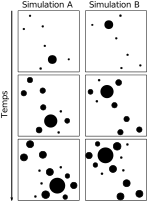
\includegraphics[width=\linewidth]{img/espace_theoriques.pdf}
		\captionsetup{width = .8\linewidth}
		\caption{Deux cas d'évolution spatio-temporelle très similaires mais non agrégables.}
		\label{fig:agreg-espace}
	\end{subfigure}
	\caption{Quelques illustrations de la difficulté de l'agrégation géographique.}
	\label{fig:agreg-geo}
\end{figure}

La situation est encore plus difficile dans le cas d'espaces théoriques moins abstraits, par exemple dans des espaces continus plutôt que discrets.
Dans la \cref{fig:agreg-espace}, on représente l'évolution de deux réplications d'un modèle théorique figurant la croissance de villes.
Les espacements, rythmes de croissances, lieux d'apparitions des nouvelles villes et l'ensemble des indicateurs sont presque identiques\footnote{
Il ne s'agit pas ici d'une simple transformation mathématique, d'où la correspondance imparfaite : les trois villes du Sud-Est dans la simulation A sont transposées dans la même configuration relative au Nord-Ouest dans la simulation B, alors que l'ensemble des autres villes subit une simple rotation de 180°.
Pour un regard de géographe, pourtant, ces deux espaces produits seront largement similaires.
}.
A nouveau, il faudrait représenter de très nombreux indicateurs pour montrer la similarité de ces deux réplications, alors qu'une planche de carte synthétise largement cette information.
Dans l'état de nos connaissances, il nous semble toutefois, à nouveau, strictement impossible d'établir une carte commune capable d'agréger l'information de ces deux réplications.
Pour le modélisateur, les deux alternatives sont donc ou bien de se contenter d'indicateurs numériques, agrégables, mais qui ne rendront pas correctement compte de la situation spatiale, ou bien de mener une observation de chacune des cartes correspondant aux différentes données produites par les réplications.

Notons que des questions du même ordre se posent même sur des données pourtant mono-dimensionnelles, par exemple avec les statistiques directionnelles (voir \cite{laloux_les_2015} par exemple).
Dans le cas des mesures d'angles, notamment, on ne peut procéder à des opérations d'agrégation classiques : la moyenne de deux angles de 30° et de 330° n'est pas de 180°, mais de 0°, ce que l'on constate immédiatement sur une rose des vents mais qui s'oppose aux logiques statistiques habituelles.

\bigskip
Cet exemple n'est pas transposable en tant que tel au problème de l'agrégation de données géographiques, de même que les obstacles soulignés dans cette partie n'ont pas de solutions claires.
Ces différents éléments permettent toutefois d'illustrer les difficultés que posent les données géographiques issues de modèles, et qui nous paraissent constituer autant de pistes de réflexion stimulantes.


\section*{Conclusion}

Le sujet de ce chapitre, la visualisation, peut sembler quelque peu décalé au regard du contenu du reste de cet ouvrage.
Nous avons toutefois souhaiter montrer à quel point l'apport de la visualisation, largement accepté vis-à-vis des données classiques, peut se révéler considérable dans le cadre de la modélisation de systèmes géographiques.
Nous postulons que chacun ne peut qu'y consentir et trouver cela évident, tant la pratique de la représentation graphique est ancrée dans la culture disciplinaire des géographes.
Nous ne pouvons pourtant, parallèlement, que constater la faiblesse de la production (carto-)graphique dans le domaine de la modélisation, quand bien même les plateformes de simulation multi-agents rivalisent de possibilités en ce sens.

Afin d'encourager les modélisateurs à s'emparer de la question de la visualisation, nous avons mis en avant les nombreuses étapes de conception d'un modèle où la visualisation peut aider le modélisateur et les spécialistes thématiciens qui l'entourent à dialoguer du modèle autour d'un cadre commun, d'une interface disciplinaire constituée par la représentation des données du modèle.
De la même manière, à l'occasion du processus d'évaluation de modèle, nous proposons une méthode, qualifiée d'évaluation visuelle, basée sur l'analyse interactive et exploratoire des données issues de simulation, toujours en vue de gagner en connaissances sur le modèle aussi bien que sur le système modélisé.
Ces acquis n'auraient pas véritablement de sens, en tout cas dans l'optique d'une démarche de cumulativité des connaissances \autocite{pumain_cumulativite_2005}, sans une capacité à les transférer à un public plus large, soit-il constitué de scientifiques, d'acteurs ou d'un public  \og profane\fg{}: la visualisation peut faciliter ce nécessaire transfert et ainsi concourir à la dissémination des apprentissages permis par les modèles.

Pour que ces apports soient complets et utiles à tous, le transfert disciplinaire ne peut être à sens unique : là où les géographes peuvent bénéficier des recherches en visualisation de données, celles-ci gagneraient aussi à affronter les problématiques propres aux données issues des modèles géographiques.
Après avoir revisité les grands principes proposés par \citefirstlastauthor{banos_pour_2013}, nous lui emprunterons ces quelques mots, en nous les ré-appropriant par le prisme de la visualisation, et en les transposant dans le contexte de la nécessaire collaboration entre géographes modélisateurs et visualisateurs de données (\citeyear[\ppno~75--76]{banos_pour_2013}): \og Nous devons prendre la place qui est la nôtre et faire valoir nos besoins dans le domaine [de la visualisation\footnote{\og du calcul intensif\fg{} dans le texte}], tout en inscrivant notre démarche dans une spirale vertueuse, au sein de laquelle disciplinarité et interdisciplinarité s'alimentent mutuellement.
Il ne suffit pas de mettre en contact des disciplines pour que l'interdisciplinarité émerge.
La pluridisciplinarité s'en contente facilement, mais l'interdisciplinarité implique des interactions entre disciplines et par conséquent une nécessaire acculturation \textelp{}
Donner les moyens aux géographes et, au delà, aux chercheurs en sciences humaines et sociales, de devenir plus autonomes dans leur démarche de [visualisation\footnote{\og modélisation\fg{} dans le texte}] va pour moi dans ce sens.\fg{}


\clearpage
\printbibliography[title={Références}]

\end{document}
